\documentclass[letterpaper,12pt]{article}
%section style
\usepackage{titletoc,tocloft}
\usepackage{breqn}
\usepackage{amssymb}
\usepackage{setspace}
\usepackage{caption}
\setstretch{1.6}
\usepackage{tabularx} % extra features for tabular environment
\usepackage{mathtools} % for 'dcases' env.
\usepackage{amsmath}  % improve math presentation
\usepackage{graphicx} % takes care of graphic including machinery
\usepackage{multirow}
\usepackage{tocloft}
\usepackage{enumerate}
\usepackage{kotex}
\usepackage{setspace}
\usepackage{caption} 
%table의 caption간격 조절하기
\captionsetup[table]{skip=5pt}
\usepackage{array}
%\usepackage{booktabs}
\usepackage{enumitem}
\usepackage{colortbl}
\usepackage{xcolor}
\usepackage{ragged2e}
\usepackage{titlesec}
%section 가운데로 설정하기.
\usepackage{sectsty}
\usepackage{upgreek}
\usepackage{algorithm}
%목차 스타일 바꾸기 
\usepackage[noend]{algpseudocode}
\sectionfont{\centering}
\usepackage[margin=1in,letterpaper]{geometry} % decreases margins
\geometry{
 a4paper,
 total={210mm,297mm},
 left=25mm,
 right=30mm,
 top=35mm,
 bottom=40mm,
 headheight=0mm,
 footskip=15mm,
 headsep=0mm,
 marginparsep=0mm,
  marginparwidth=0mm,
  bindingoffset=0mm
 }
\usepackage{indentfirst}\setlength\parindent{1em} %문단 들여쓰기 하는 거 
%들여쓰기를 하고싶지 않은 문단에는 앞머리에 \noindent
% \usepackage{cite} % takes care of citations
% \usepackage{biblatex} %Imports biblatex package
% \addbibresource{Ref.bib} %Import the bibliography file
% \usepackage[final]{hyperref} % adds hyper links inside the generated pdf file
% \hypersetup{
%   colorlinks=true,       % false: boxed links; true: colored links
%   linkcolor=blue,        % color of internal links
%   citecolor=blue,        % color of links to bibliography
%   filecolor=magenta,     % color of file links
%   urlcolor=blue         
% }
\usepackage{amsmath}
\usepackage{blindtext}
\usepackage{graphics, graphicx,multirow,enumerate}
\usepackage[authoryear,sort]{natbib}
\usepackage[font=small]{caption}
\usepackage{subcaption}
 \usepackage{booktabs}

\begin{document}

%%
%%%%%%%%%%%%%%%%%%%%%%%%% 첫표지
\thispagestyle{empty}
\vspace{4.5cm}
\begin{center}
\fontsize{16}{60} \selectfont{석 사 학 위 논 문\\}
\vspace{2cm}
\fontsize{22}{25} \selectfont{
단일 문서 내 복수 작성자 탐지를 위한\\
MIL 기반 필적 분석\\}
\vspace{8cm}
\fontsize{16}{10} \selectfont{양 덕 관\\ 
}
\vspace{2cm}
\fontsize{16}{15} \selectfont{
부산대학교 대학원 \\}
\vspace{0.5cm}
\fontsize{16}{15} \selectfont{통계학과\\}
\vspace{2cm}
\fontsize{16}{10} \selectfont{2026년 2월\\}


\end{center}

\newpage
\thispagestyle{empty}
\begin{center}
\vspace{4.5cm}
\fontsize{0.1}{1} \selectfont{ㅁ}
\end{center}

\newpage
\thispagestyle{empty}
\begin{center}
\vspace{4cm}
\fontsize{22}{12} \selectfont{
단일 문서 내 복수 작성자 탐지를 위한\\
MIL 기반 필적 분석 \\}
\vspace{1.5cm}
\fontsize{16}{10} \selectfont{이 논문을 이학석사 학위논문으로 제출함\\}
\vspace{1.0cm}
\fontsize{14}{10} \selectfont{양 덕 관 \\}
\vspace{1.0cm}
\fontsize{14}{10} \selectfont{부산대학교 대학원\\}
\vspace{0.5cm}
\fontsize{14}{10} \selectfont{통 계 학 과 \\}
\vspace{1.0cm}
\fontsize{14}{10} \selectfont{지 도 교 수 박 소 영 \\}
\vspace{5.5cm}
\fontsize{16}{12} \selectfont{양덕관의 이학석사 학위논문을 인준함\\}
\vspace{1cm}
\fontsize{14}{12} \selectfont{2025년 12월 31일\\}
\vspace{1cm}
\begin{table}[H]
\fontsize{14}{12} \selectfont
\renewcommand{\arraystretch}{1.2}
\renewcommand{\tabcolsep}{5mm}
\centering
\begin{tabular}{lclll}
위원장  & 홍 길 동 &  &  &  \\ \cline{4-5} 
위 원 & 홍 길 동   &  &  &  \\ \cline{4-5} 
위 원 & 홍 길 동  &  &  &  \\ \cline{4-5} 
\end{tabular}
\end{table}
\end{center}


%%%%%%%%%%%%%%%%%%%%%%%%%5 목차 직접생성 

%\parskip.2cm
%\parindent1.1cm

\newpage
 \newgeometry{
 a4paper,
 total={210mm,297mm},
 left=25mm,
 right=30mm,
 top=35mm,
 bottom=40mm,
 headheight=0mm,
 footskip=15mm,
  headsep=0mm,
  headheight=0mm,
  marginparsep=0mm,
  marginparwidth=0mm,
   bindingoffset=0mm
}


\renewcommand{\thepage}{\roman{page}}
\setcounter{page}{1}




\centerline{\LARGE \bf 목차}

\begin{flushright}
    page
\end{flushright}

% \vspace{2mm} \noindent {\normalsize \bf List of Tables} \dotfill ii\

% \vspace{2mm} \noindent {\normalsize \bf List of Figures} \dotfill iii\

% \vspace{2mm} \noindent {\normalsize \bf Abstract} \dotfill v\

\vspace{2mm} \noindent {\normalsize \bf 1. 서론} \dotfill 1

\vspace{1mm} \noindent {\normalsize \bf 2. 배경지식} \dotfill 3

\vspace{-0.2cm}\parindent1.86cm{\bf 2.1 Huber's $M$-estimation } \dotfill 4

\vspace{-0.2cm}\parindent1.86cm{\bf 2.2 $M$-Smoother } \dotfill 5

\vspace{-0.2cm}\parindent1.86cm{\bf 2.3 Moving Huber $M$-estimation } \dotfill 6

\vspace{-0.2cm}\parindent1.86cm{\bf 2.4 Comparison } \dotfill 6

\vspace{-0.2cm}\parindent1.86cm{\bf 2.5 Scale parameter \& Loss Function } \dotfill 8


\vspace{1mm} \noindent {\normalsize \bf 3. 모의실험 } \dotfill 14

\vspace{1mm} \noindent {\normalsize \bf 4. 실제 데이터 } \dotfill 17

\vspace{-0.2cm}\parindent1.86cm{\bf 4.1 2021년도 게임스탑 고가 데이터 } \dotfill 17

\vspace{-0.2cm}\parindent1.86cm{\bf 4.2 도로 교통 센서 점유율 } \dotfill 19

\vspace{-0.2cm}\parindent1.86cm{\bf 4.3 트위터 언급량 } \dotfill 21

\vspace{1mm} \noindent {\normalsize \bf 5. 결론 } \dotfill 23

\vspace{1mm} \noindent {\normalsize \bf References} \dotfill 24


% \noindent {\normalsize \bf Abstract(in Korean)} \dotfill 34

\newpage
\centerline{\LARGE \bf 표 목차}

\vspace{3mm}
\noindent
\begin{tabular*}{\textwidth}{@{\extracolsep{\fill}}p{0.9\textwidth}r}
\textbf{표 1: 점프 데이터에서의 성능지표($\sigma$ = 1, window = 5)} & 11 \\
\end{tabular*}
\vspace{3mm}
\begin{tabular*}{\textwidth}{@{\extracolsep{\fill}}p{0.9\textwidth}r}
\textbf{표 2: 점프 데이터에서의 성능지표($\sigma$ = 1, window = 101)} & 11 \\
\end{tabular*}
\vspace{3mm}
\begin{tabular*}{\textwidth}{@{\extracolsep{\fill}}p{0.9\textwidth}r}
\textbf{표 3: 점프 데이터에서의 성능지표($\sigma$ = 10, window = 5)} & 12 \\
\end{tabular*}
\vspace{3mm}
\begin{tabular*}{\textwidth}{@{\extracolsep{\fill}}p{0.9\textwidth}r}
\textbf{표 4: 점프 데이터에서의 성능지표($\sigma$ = 10, window = 101)} & 12 \\
\end{tabular*}
\vspace{3mm}
\begin{tabular*}{\textwidth}{@{\extracolsep{\fill}}p{0.9\textwidth}r}
\textbf{표 5: 점프 데이터에서의 성능지표($\sigma$ = 20, window = 5))} & 13 \\
\end{tabular*}
\vspace{3mm}
\begin{tabular*}{\textwidth}{@{\extracolsep{\fill}}p{0.9\textwidth}r}
\textbf{표 6: 점프 데이터에서의 성능지표($\sigma$ = 20, window = 101)} & 13 \\
\end{tabular*}
\vspace{3mm}
\begin{tabular*}{\textwidth}{@{\extracolsep{\fill}}p{0.9\textwidth}r}
\textbf{표 7: $\sigma$ = 0.05, Model 1(엣지가 있는 신호에 가우시안 노이즈)} & 16 \\
\end{tabular*}
\vspace{3mm}
\begin{tabular*}{\textwidth}{@{\extracolsep{\fill}}p{0.9\textwidth}r}
\textbf{표 8: $\sigma$ = 0.05, Model 5(부드러운 신호에 가우시안 노이즈)} & 16 \\
\end{tabular*}
\vspace{3mm}
\begin{tabular*}{\textwidth}{@{\extracolsep{\fill}}p{0.9\textwidth}r}
\textbf{표 9: $\sigma$ = 0.5, Model 8(부드러운 신호에 코시 노이즈)} & 16 \\
\end{tabular*}
\vspace{3mm}


\newpage
\newpage
\begin{center}
\LARGE \bf 그림 목차
\end{center}

\vspace{3mm}
\noindent
\begin{tabular*}{\textwidth}{@{\extracolsep{\fill}}p{0.9\textwidth}r}
\textbf{그림 1: 이동평균의 과도한 평활화 } & 1 \\
\end{tabular*}

\vspace{3mm}
\noindent
\begin{tabular*}{\textwidth}{@{\extracolsep{\fill}}p{0.9\textwidth}r}
\textbf{그림 2: 점프 데이터에서의 세 가지 디노이징 방법들의 비교; (a) 윈도우 크기 5, (b) 51, (c) 101 } & 7 \\
\end{tabular*}

\vspace{3mm}
\noindent
\begin{tabular*}{\textwidth}{@{\extracolsep{\fill}}p{0.9\textwidth}r}
\textbf{그림 3: 점프 데이터에서 MH의 세 가지 척도모수 추정 방법들의 비교; (a) 윈도우 크기 5, (b) 51, (c) 101 } & 8 \\
\end{tabular*}

\vspace{3mm}
\noindent
\begin{tabular*}{\textwidth}{@{\extracolsep{\fill}}p{0.9\textwidth}r}
\textbf{그림 4: 두가지 형태의 신호.(왼쪽) 엣지가 있는 신호, (오른쪽) 부드러운 신호 } & 14 \\
\end{tabular*}

\vspace{3mm}
\noindent
\begin{tabular*}{\textwidth}{@{\extracolsep{\fill}}p{0.9\textwidth}r}
\textbf{그림 5: 게임스탑 고가 그래프} & 18 \\
\end{tabular*}

\vspace{3mm}
\noindent
\begin{tabular*}{\textwidth}{@{\extracolsep{\fill}}p{0.9\textwidth}r}
\textbf{그림 6: 도로 교통 센서 점유율 그래프 } & 20 \\
\end{tabular*}

\vspace{3mm}
\noindent
\begin{tabular*}{\textwidth}{@{\extracolsep{\fill}}p{0.9\textwidth}r}
\textbf{그림 7: 트위터 언급량 그래프 } & 22 \\
\end{tabular*}



%%%%%%%%%%%%%%%%%%
%%%%%%%%%%%%%%%% 목차생성 끝

%%%%%%%%%%%%%%%%%%%%%%% Abstract
%\newpage
%\setlength{\cftsecindent}{1em}
%\setlength{\cftsubsecindent}{5.5em}
\renewcommand\thesection{\arabic{section}.}
%\makeatletter
%   \renewcommand \l@section{\@dottedtocline{1}{1.5em}{5em}}
%%%\makeatother
 \renewcommand\thesubsection{\arabic{section}.\arabic{subsection}}
%\newpage
%\tableofcontents
%\addtocontents{toc}{~\hfill\textbf{Page}\par}
%\renewcommand{\cftsecfont}{\Large\itshape}
%%\vspace{1.5cm}
%\listoffigures
%%\renewcommand{\thepage}{\roman{page}}
%\setcounter{page}{1}
%%
\newpage
\begin{center}
\vspace{3.5cm}
\fontsize{14}{10} \selectfont{
단일 문서 내 복수 작성자 탐지를 위한 MIL 기반 필적 분석\\}
\vspace{1.5cm}
\fontsize{12}{10} \selectfont{김 동 혁\\}
\vspace{1cm}
\fontsize{11}{10} \selectfont{부산대학교 대학원 통계학과\\}
\vspace{1.5cm}
\fontsize{12}{10} \selectfont{요약\\}
\vspace{-\baselineskip}
\end{center}
\vspace{1cm}
\fontsize{11}{10} \selectfont{

\setlength{\parindent}{1em}
본 연구는 경계와 이상점이 많은 시계열 신호에서 이동평균(MA)의 과도한 평활화 문제와 이동중앙값(MM)의 계산비용·확장성 한계를 보완할 대안을 탐색하기 위해, 로버스트 방법과의 비교와 데이터 유형별 선택 지침 확립을 목적으로 한다. 이를 위해 이미지 분야에서 제안된 $M$-smoother 아이디어와 Huber $M$-estimation의 IRLS(Iteratively Reweighted Least Squares) 절차를 창 기반으로 적용한 Moving Huber $M$-estimation(MH)을 정의하고, MA·MM·단순지수평활법(SES)과 함께 비교하였다. 모의실험은 (i) 경계가 많은 신호와 (ii) 부드러운 선형 신호를 구성한 뒤, 가우시안·라플라스·가우시안 혼합·코시 등 네 가지 노이즈를 추가하여 $L_1,L_2,L_\infty$ 지표로 성능을 평가하였고, 외삽 가능성 평가는 실제 데이터(2021년 GameStop 일별 고가, 도로 교통 센서 점유율, 트위터 ‘GOOG’ 언급량)에 적용해 확인하였다. 그 결과, 신호 구조와 노이즈 특성에 따라 최적 방법이 달라짐이 확인했다. 신호에 경계가 존재하며 노이즈 수준이 낮을때 MH 기반 방법들이 우수한 성능을 보여줬고, 신호가 경계 없이 부드럽게 변하는 경우에는 단순지수평활법이 성능이 가장 좋았다. 또한 코시 분포와 비슷한 환경에서는 이동중앙값이 뛰어난 성능을 보여주었다. 결론적으로 단일 방법의 보편적 우위는 없으며, 신호의 유형을 고려한 선택이 필요하고, MA와 MM의 장단점을 보완하는 실용적 대안으로서 창 기반 MH의 적용 가능성을 제안한다.


% Chap 1
\newpage
\restoregeometry
\section{서론}
\renewcommand{\thepage}{\arabic{page}}
\setcounter{page}{1}
\setlength{\parindent}{1em}

시계열 데이터(time series data)는 주가, 기온, 신호 데이터 등 시간 순서에 따라 측정되는 데이터로서, 다양한 분야에서 분석이 요구된다\citep{box2015timeseries}. 그러나 관측 과정에서 잡음(noise)과 이상점(outlier)이 불가피하게 포함되는데, 이는 잘못된 결론을 도출하게 하는 요인 중 하나이다. 따라서 이상점의 효과를 덜 영향을 받으며, 기존의 시계열 패턴을 보존하는 디노이징(denoising) 방법은 매우 중요하다.

시계열 분석에서 가장 많이 사용되는 이동평균(moving mverage, MA) 방법은 연산이 간단하고 계산속도가 매우 빠르다는 장점이 있지만, Figure 1과 같이 급격한 변화가 있는 영역인 경계(boundary)나 이상점을 과도하게 평활화(smoothing)하는데 이는 정보 손실의 우려가 있다.
\begin{figure}[H]
    \centering
    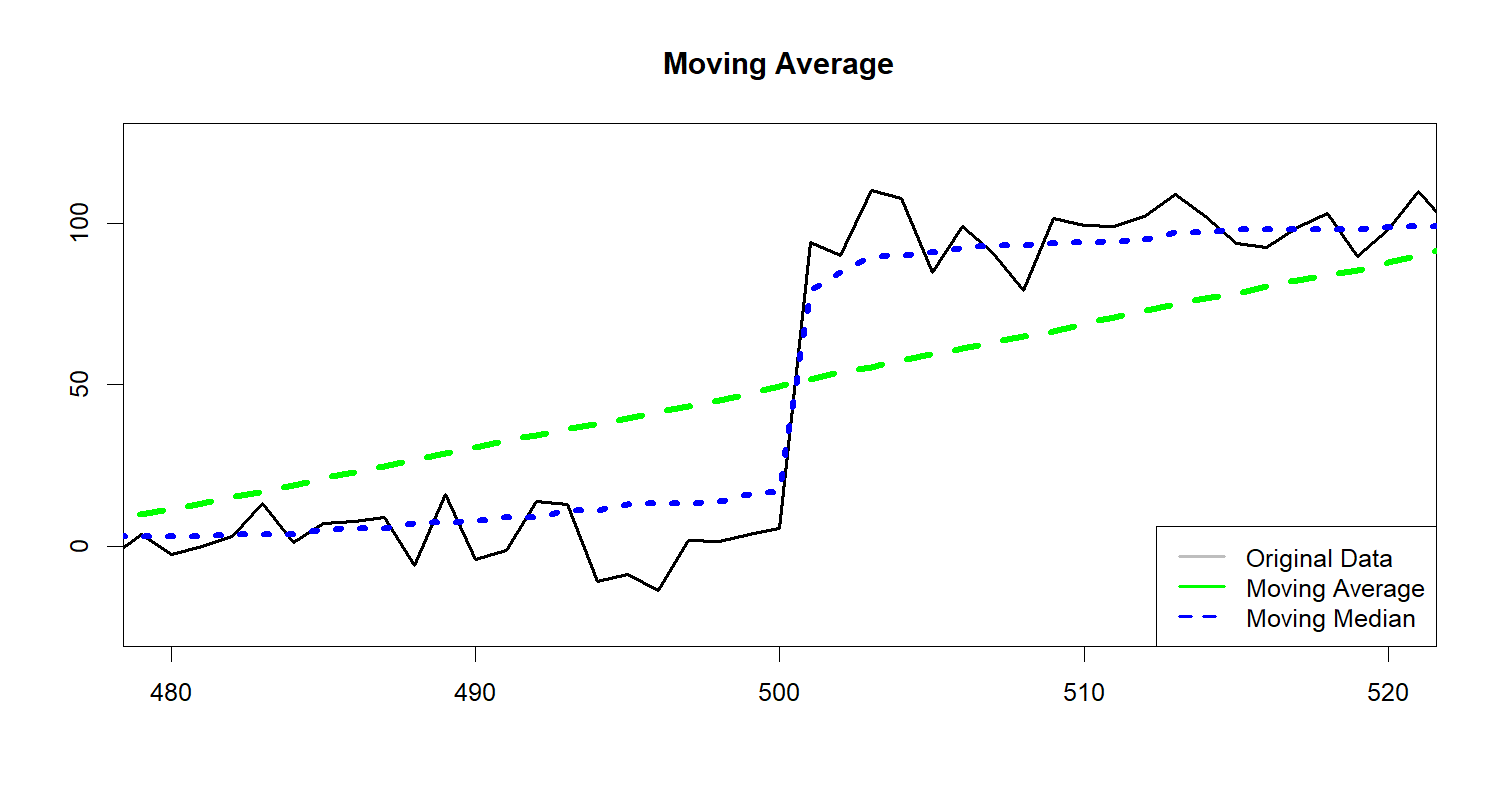
\includegraphics[width=0.8\linewidth]{figures/MAMM.png}
    \caption{이동평균의 과도한 평활화}
\end{figure}
반면에, 이동중앙값(moving median, MM)은 이상점을 효과적으로 배제하거나 완화시킬 수 있다. 또한, 이동평균 필터와 달리 데이터의 급격한 변화 지점인 경계(boundary)를  Figure 1 처럼 흐리게 만들지 않고 보존하는 데 강점이 있다. 이 덕분에 데이터의 원래 형태를 유지하면서 점잡음(salt-and-pepper noise)를 제거하는 데 매우 효과적이다. 하지만, 데이터 크기가 커질수록 계산량이 급등하므로 계산의 효율이 낮아질 수 있다\citep{huang1979fast}.

이에 본 연구에서는 경계 보존에 효과적인 로버스트 방법인 \citet{huber1981robust}의 $M$-estimation을 시계열 데이터에 적용하고자 한다. 구체적으로는 Huber loss를 활용한 Huber location 추정 방식을 창을 따라 움직이는 방식을 사용하며, 이를 편의상 Moving Huber $M$-estimation(MH)라고 명명한다. 본 연구는 Moving Huber $M$-estimation를 선형 구조(linear structure)와 경계 데이터(boundary data) 등 시계열 데이터에 디노이징을 적용함으로써 이동평균과 이동중앙값이 가지는 한계를 보완하고, 이상점이 존재하는 복잡한 시계열 환경에서 방법들을 비교해보려고 한다.





%%%%%%%%%%%%%%%%%%%%%%%%%%%%%%%%%%%%%%%%%%%%%%%%%%%%
\clearpage
%% Chap 2
%% Chap 2
\section{배경지식}\label{sec:setup}
본 논문에서는 시계열 데이터의 디노이징을 위해 네 가지 방법을 사용하였다. 현재 평활화 방법 중 가장 널리 쓰이고 있는 이동평균과 이상점 감지에 유용하게 쓰이는 이동중앙값, 간단하고 직관적인 단순지수평활법(simple exponential smoothing, SES), 마지막으로 Moving Huber $M$-estimation이다.

이동평균은 일정 구간 $W$의 데이터 값들의 평균을 계산하여, 해당 구간을 대표하는 값으로 사용하는 방법이다. 가장 많이 알려져 있어, 라이브러리에서 기본적으로 제공하여 현업이나 분석과정에서 적용하기 쉽다. 계산이 덧셈, 뺄셈만으로 이루어져 있어 계산 속도 또한 매우 빠르다. 하지만, 경계 데이터에서 급격한 변화를 과하게 평활화하기 때문에 세부정보를 놓칠 가능성이 있다.


아울러, 데이터에 이상점이 있을 경우 민감하게 반응하여 왜곡이 커질 수 있다. 이동평균 방법 중 단순 이동평균, 이중 이동평균 등 여러가지 방법이 있는데 본 논문에서는 단순 중심이동평균을 사용하여 아래의 식에 표현하였다.

\[
MA_T = (Y_{T - \frac{W-1}{2}} + \dots + Y_T +\dots + Y_{T + \frac{W-1}{2}})/W
\]

$T$는 시점, $W$는 창 크기, $Y$는 기존 시계열 데이터, $MA_T$는 시점 $T$에서의 창 크기 $W$만큼을 평균낸 값이다. 창은 $T$시점을 중심으로 과거와 미래에 각각 동일한 간격 $(W-1)/2$만큼 떨어지게 설정했다. 그러므로, $W$는 홀수 값만 가능하다.

이동중앙값은 일정 구간 $W$의 중앙값을 대표값으로 사용하는 방법이다. 이동중앙값은 이상점에 로버스트하고 경계 데이터의 급격한 지역적 변화를 비교적 잘 보존한다. 하지만, 구간마다 데이터를 정렬해야하는데 이는 이동평균보다 계산비용이 더 많다. 즉, 데이터 또는 창 크기가 커질수록 이동평균보다 계산비용이 더 많아진다. 아래는 이동중앙값을 산출하는 식이다.

\[
MM_T = \mbox{median}(Y_{T - \frac{W-1}{2}} , \dots , Y_T , \dots , Y_{T + \frac{W-1}{2}})
\]

단순지수평활법은 이동평균, 이동중앙값과 달리 창을 사용하지 않고 과거의 관측값에 지수적으로 감소하는 가중치를 부여해 미래를 예측하는 방식이다. 경계와 같은 급격한 수준 변화가 발생했을 때, 단순지수평활법은 그 변화를 서서히 따라가기 때문에 실제 변화보다 항상 뒤처지는 특성을 보인다. 이는 경계 전후의 평활화 곡선이 왜곡되는 결과를 낳는다. 계산 비용이 적어서 실시간 처리에 적합하지만, 추세나 주기적인 패턴이 있을 경우 예측력이 낮아질 수 있다.
\[
ES_T= \alpha Y_{T-1} +(1-\alpha)ES_{T-1} , (0<\alpha<1)
\]
이때 $Y_{T-1}$은 $T-1$시점의 시계열 데이터, $ES_T$는 $T-1$시점에서 다음값 $Y_T$의 예측값이다. 

이러한 고전적 방법들의 문제는 경계를 보존하면서도 효율적으로 잡음을 제거할 새로운 로버스트 방법론의 필요성을 절감하게 했다. 이런 배경 속에서 경계 보존 평활화의 초기 접근 방식들이 이미치 처리 분야에서 등장했다. 
\cite{lee1983digital}가 제안한 시그마 필터는 국소 가중 ��균의 개���을 확장하여, 경계를 넘어선 평활화를 방지했다. 특히 \cite{chu1998edge}가 제안한 $M$-smoother는 로버스트한 $M$-estimation 아이디어를 도입하면서 경계 보존에 결정적인 통찰을 제시했다. $M$-smoother는 $M$-함수의 국소 최솟값을 활용하여 평활화 결과를 결정하는데, 이 국소 최솟값을 이용하는 것이 경계 보존 평활화에 핵심적인 효과가 있음이 입증되었다. 일반적으로 하나의 전역 최솟값을 가져야하지만, 국소적인 경향을 나타내는 최솟값이 여러 개면 경계 전후의 서로 다른 평활화된 값을 나타내는 핵심적인 역할을 한다.

이러한 로버스트 $M$-estimation 기반의 국소 최소 탐색 통찰은 경계 보존 평활화가 이상점 뿐만 아니라 구조적 불연속성에도 강건하게 작동할 수 있는 기반을 마련했다. 따라서 본 연구는 이 성공적인 배경을 바탕으로 $M$-estimation을 시계열 데이터에 적용하는 방법을 탐구하게 되었다.

%%% Chap 2.1
\subsection{Huber's $M$-estimation}\label{sec:setup}


\citet{huber1981robust}는 데이터에 존재하는 이상점의 영향을 줄이면서 로버스트하게 모수를 추정하기 위한 최우추정(maximum likelihood)의 일반화된 방법으로 $M$-estimation을 제안했다.  잔차에 대한 손실함수 $\rho(r_i)$의 합을 최소화하여 $\theta$의 추정치를 구한다. 

\[
\hat{\theta} = \arg\min_{\theta} \sum_{i=1}^n \rho(r_i),       r_i=\frac{x_i-\theta}{s}
\]
이때 $s$는 척도 모수(scale parameter)로, 주로 중앙절대편차(median absolute deviation, MAD)를 사용한다. 후버손실함수(huber loss function) $\rho$는 다음과 같이 주어진다.
\[
\rho_c(r) =
\begin{cases} 
\frac{r^2}{2}, & \text{if } |r| \leq c, \\ 
c \left( |r| - \frac{c}{2} \right), & \text{if } |r| > c.
\end{cases}
\]
잔차가 임계값 $c$보다 작은 경우에는 제곱 손실을 사용하고, $c$ 이상인 경우에는 절댓값 손실 함수를 사용한다. 그리고 이 함수를 미분한 $\psi_c(r)$함수는 
 \[
\psi_c(r) =
\begin{cases} 
r, & \text{if } |r| \leq c, \\ 
c \, \mathrm{sign}(r), & \text{if } |r| > c.
\end{cases}
\]
추정값을 업데이트 할 때 사용한다. 이때 sign($r$)은 부호함수로, 
\[
\operatorname{sign}(r) =
\begin{cases}
+1, & r>0,\\
0,  & r=0,\\
-1, & r<0.
\end{cases}
\]
를 의미한다.
그런 $\psi$함수에 잔차 $r_i$를 나눈 값을 가중치로 사용하는데,
 \[
w_i = \frac{\psi_c(r_i)}{r_i} =
\begin{cases} 
1, & \text{if } |r_i| \leq c, \\ 
\frac{c}{|r_i|}, & \text{if } |r_i| > c.
\end{cases}
\]
잔차가 특정거리 $c$ 안에 있으면 1의 값을, $c$ 보다 멀어질수록 거리에 반비례하는 가중치를 갖는다. 

위치-척도(location-scale)모형에서 M-estimation을 하는 방법은 다음과 같다. 먼저 초기 추정값 $\theta^{(0)}$을 데이터의 평균이나 중앙값 등으로 설정한다. $t$번째 에서의 잔차 $r_i^{(t)}$를 계산하고 그에 따라 가중치 $w_i^{(t)}$를 계산한다. 그리고 IRLS 방법을 통해 다음 $t+1$번째 추정값 $\theta^{(t+1)}$를 계산한다. $t+1$번째와 $t$번째 추정값의의 차이가 주어진 threshold인 $\epsilon$보다 작거나 $t$가 max iteration인 $t^{max}$ 보다 커지면 알고리즘을 종료한다.


\begin{algorithm}[H]
\caption{Iteratively Reweighted Least Squares (IRLS) for $M$-estimation}
\label{alg:StoTheta}
    \begin{algorithmic}
        \State 1: $\theta^{(0)}$
        \State 2: $r_i^{(t)} = \frac{x_i - \theta^{(t)}}{s}$ 
        \State 3: $w_i^{(t)} = \min\left( 1, \frac{c}{|r_i^{(t)}|} \right)$
        \State 4: $\theta^{(t+1)} = \frac{\sum_{i=1}^n w_i^{(t)} x_i}{\sum_{i=1}^n w_i^{(t)}}$
        \State 5: stop when $\left| \theta^{(t+1)} - \theta^{(t)} \right| < \varepsilon$ or $t \geq t^{max}$
    \end{algorithmic}
\end{algorithm}




%%% Chap 2.3

\subsection{Moving Huber $M$-estimation}\label{sec:setup}
$M$-Smoother는 점 추정이 아닌, 구간을 움직이면서 국소 최소값을 선택하는 방식이었다. 하지만 $M$-estimation을 그대로 구현한 것이 아니라 이미지 처리 분야에 맞게 식을 변형해서 사용했다. 본 논문에서는 기존의 $M$-estimation 점 추정 방법을 시계열 데이터에 그대로 적용하려고 한다. 먼저 $\rho(\cdot)$를 Huber 손실함수로 사용하고, 거기에 곱해져 있는 커널함수를
\[
K_h(x-x_j)=
\begin{cases}
    1 , & \text{if } |x-x_j|<h \\
    0 , & \text{if } |x-x_j|>h
\end{cases}
\]
로 사용한다.

%%% Chap 2.4

\subsection{Comparison}\label{sec:setup}

앞 절에서 소개한 Huber의 $M$-estimation을 시계열 데이터에 적용하여 이동평균과 이동중앙값 방법과 비교했다. 시점은 1부터 1000까지고, 500전까지는 평균이 0이고 표준편차가 10인 가우시안 노이즈이며, 500번째 시점에서 100의 값으로 점프하여 그 상태를 유지하는 데이터이다. 편의상 $x$축 450에서 550까지만 나타냈으며, Figure1의 (a)는 창을 5, (b)는 51, (c)는 101로 놓고 실험하였다.
\begin{figure}[H]
    \centering
    \begin{subfigure}[b]{\linewidth}
        \centering
        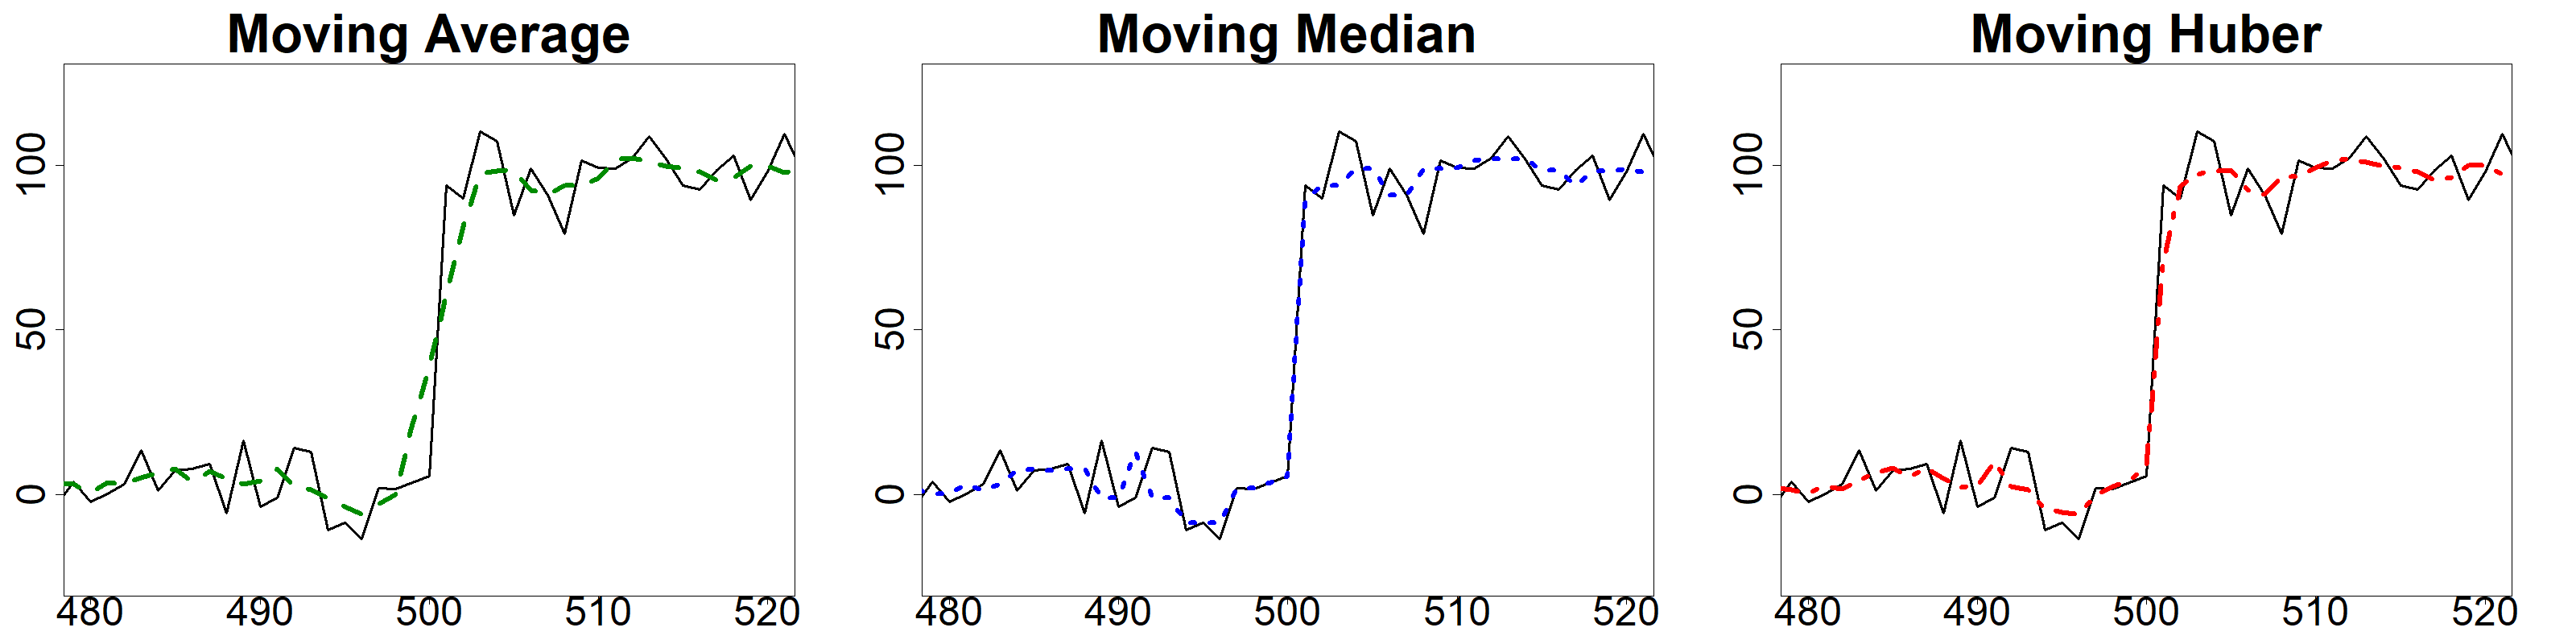
\includegraphics[width=\linewidth]{figures/3comparison5.png}
        \caption{}
    \end{subfigure}
    
     \vspace{1em}
    
    \begin{subfigure}[b]{\linewidth}
        \centering
        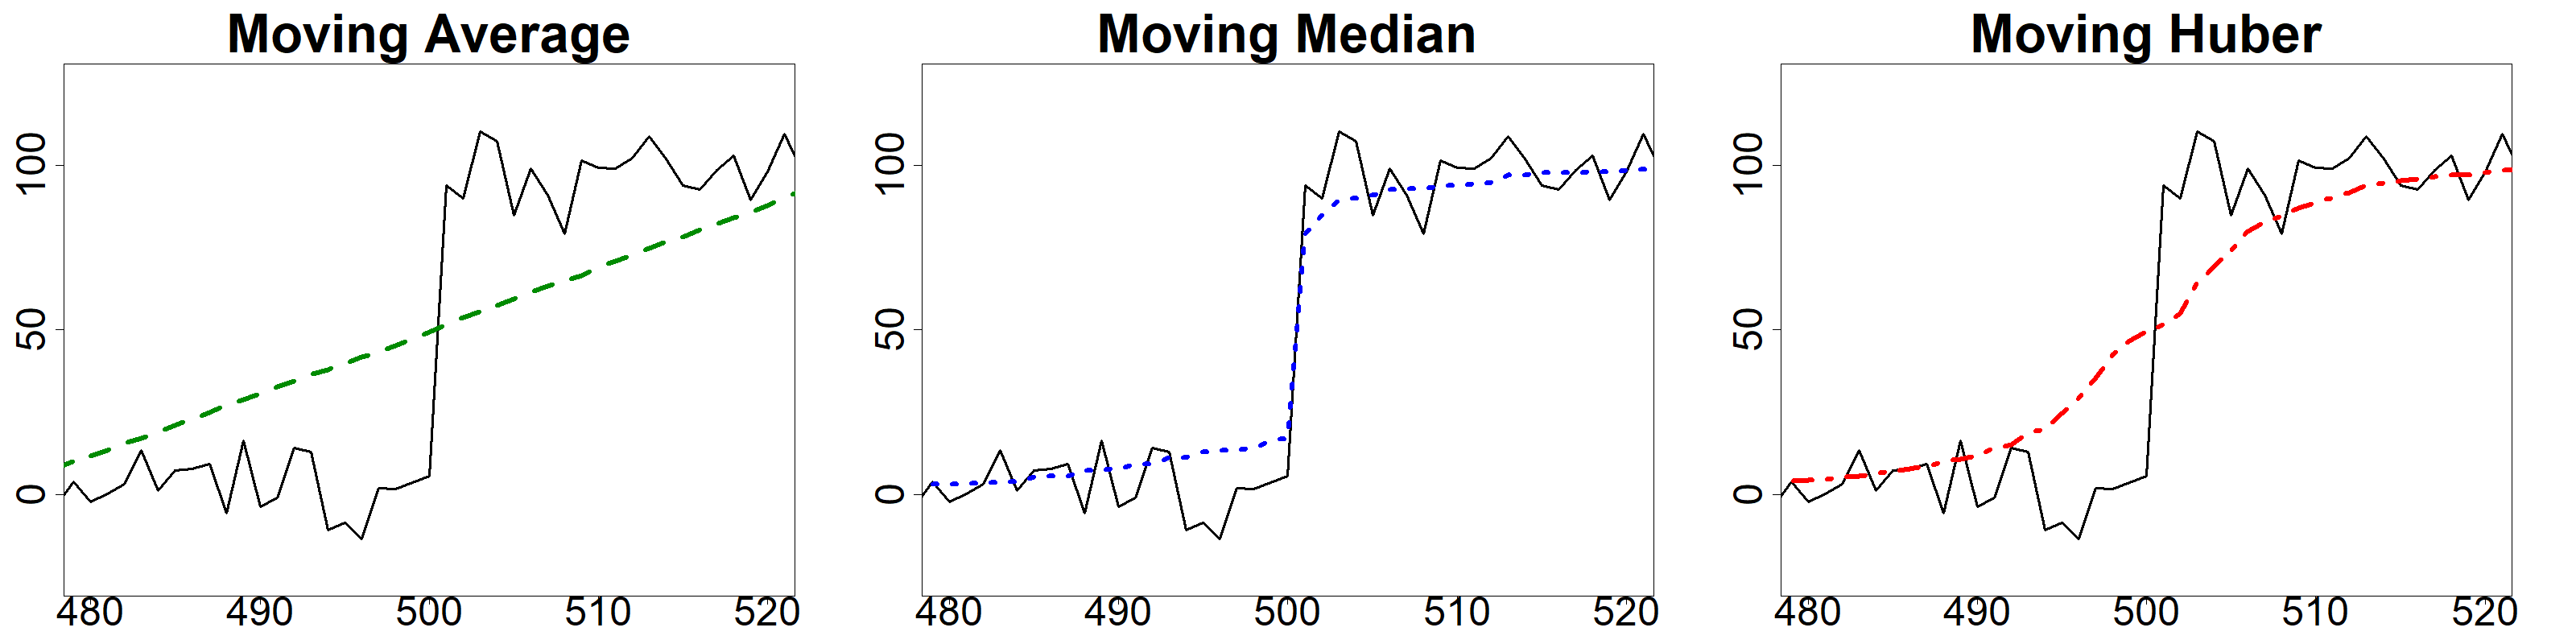
\includegraphics[width=\linewidth]{figures/3comparison51.png}
        \caption{}
    \end{subfigure}
       
    \vspace{1em}
    
    \begin{subfigure}[b]{\linewidth}
        \centering
        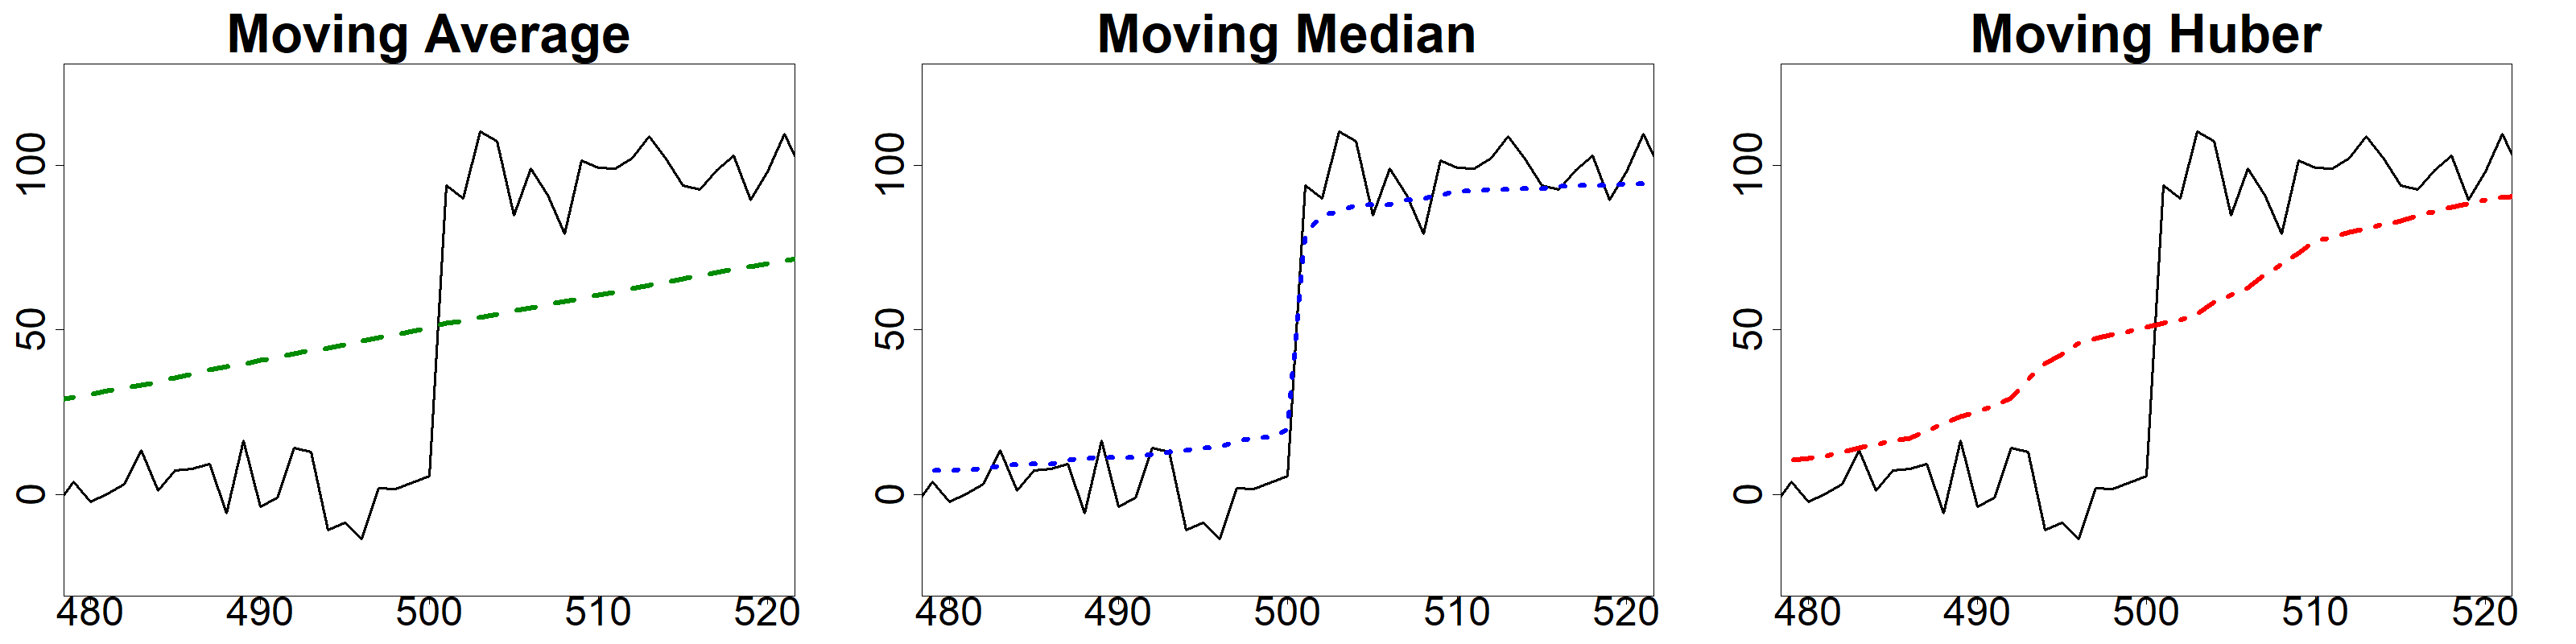
\includegraphics[width=\linewidth]{figures/3comparison101.png}
        \caption{}
    \end{subfigure}
    
    \caption{점프가 있는 모의실험 데이터에서의 세 가지 방법들의 비교; (a) 창 크기 5, (b) 51, (c) 101.}
    \label{fig:comparison}
\end{figure}
Figure 2(a)에서, 점프 밖의 구간에 대해서는 세 가지 방법들이 유사하게 디노이징을 했다. 하지만 점프가 있는 [495,505] 구간에서는 이동평균이 가장 평활하게 추정하며 점프라는 정보를 평활화했으며, 이동중앙값은 매우 로버스트하게 작동하여 점프를 가장 유사하게 나타냈다. 반면 MH는 그 둘 사이의 중앙에 위치하면서도 곡선의 형태를 나타냈다. 너무 로버스트하지도 않고 너무 평활하지도 않다.
Figure 2(b),(c)에서와 같이 큰 창에서는 이동평균은 잘 평활시키는 모습을 볼 수 있으며, 이동중앙값은 Figure 2(a)보단 정도가 약해졌지만 여전히 점프라는 특징을 잘 잡아내고 있다. 여기서 MH는 점진적으로 상승하는 곡선의 형태를 나타냈다.







%%% Chap 2.5
\subsection{Scale parameter \& Loss Function}\label{sec:setup}
Huber의 M-estimation는 이상점의 영향을 최소화하는 강인한 추정을 목적으로 하므로, 척도 모수를 추정할 때에도 강인한 방법인 MAD를 주로 쓴다.
MAD는 중앙절대편차로, 다음식과 같이 중앙값을 2번 사용하는 방법이다.
\[
\mbox{MAD}(x)= \mbox{median}(|X_i-\mbox{median}(X)|)
\]


\begin{figure}[H]
    \centering
    \begin{subfigure}[b]{\linewidth}
        \centering
        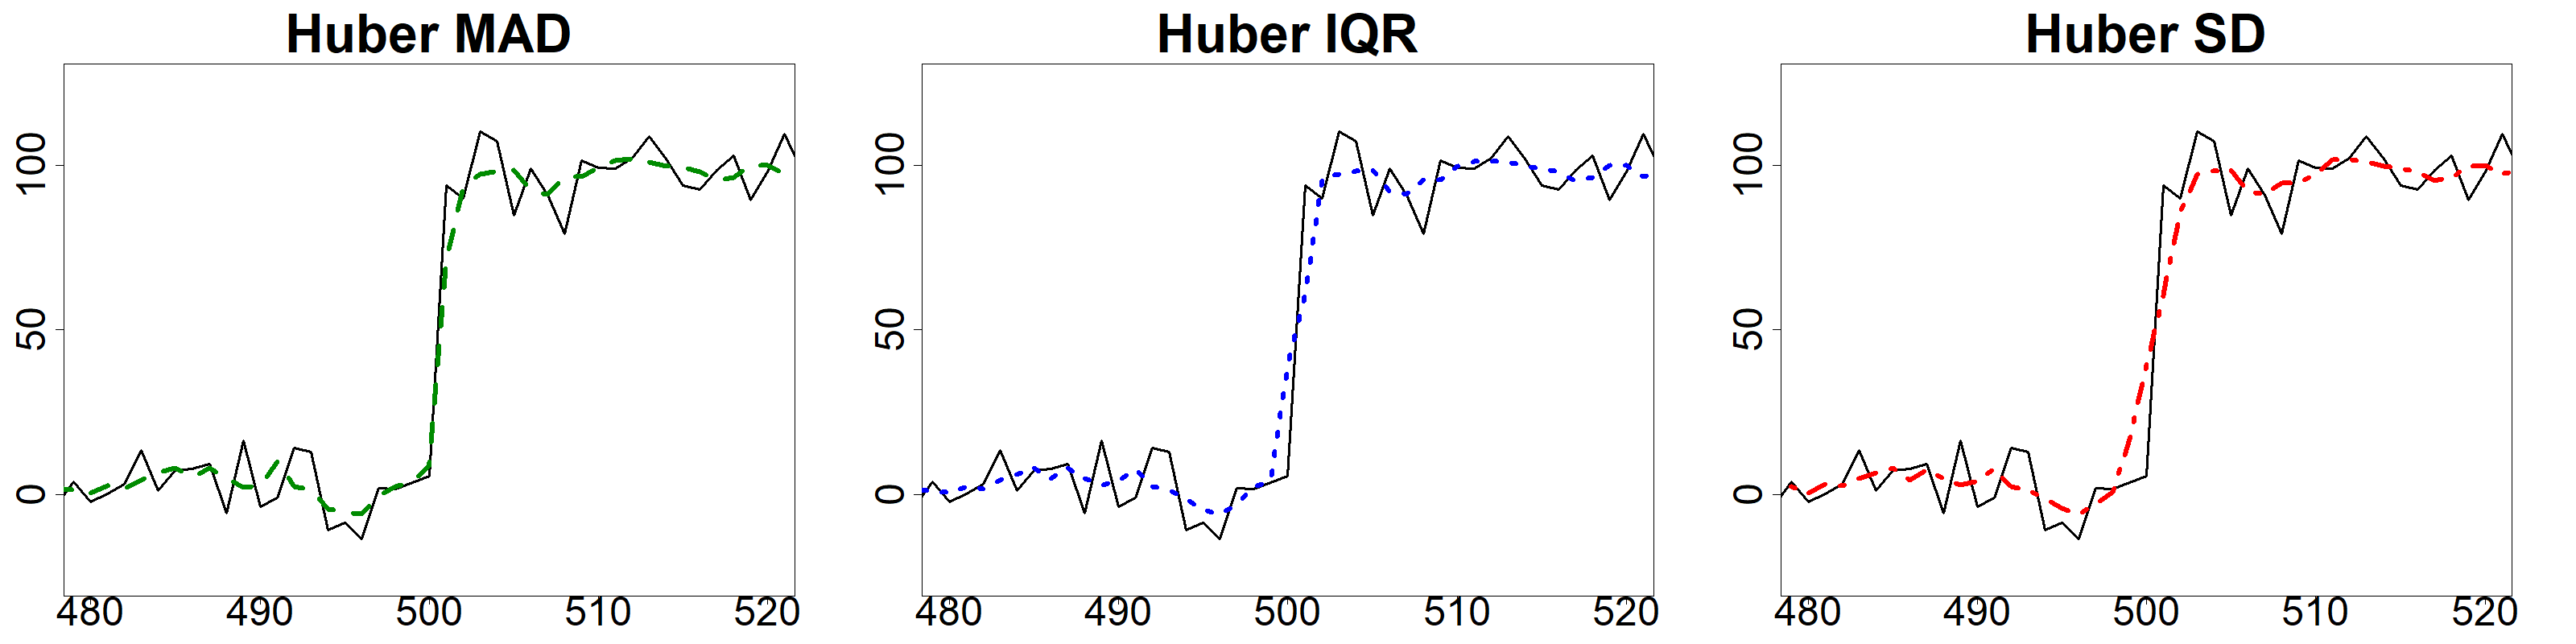
\includegraphics[width=\linewidth]{figures/3scale5.png}
        \caption{}
    \end{subfigure}
    
    \vspace{1em}
    
    \begin{subfigure}[b]{\linewidth}
        \centering
        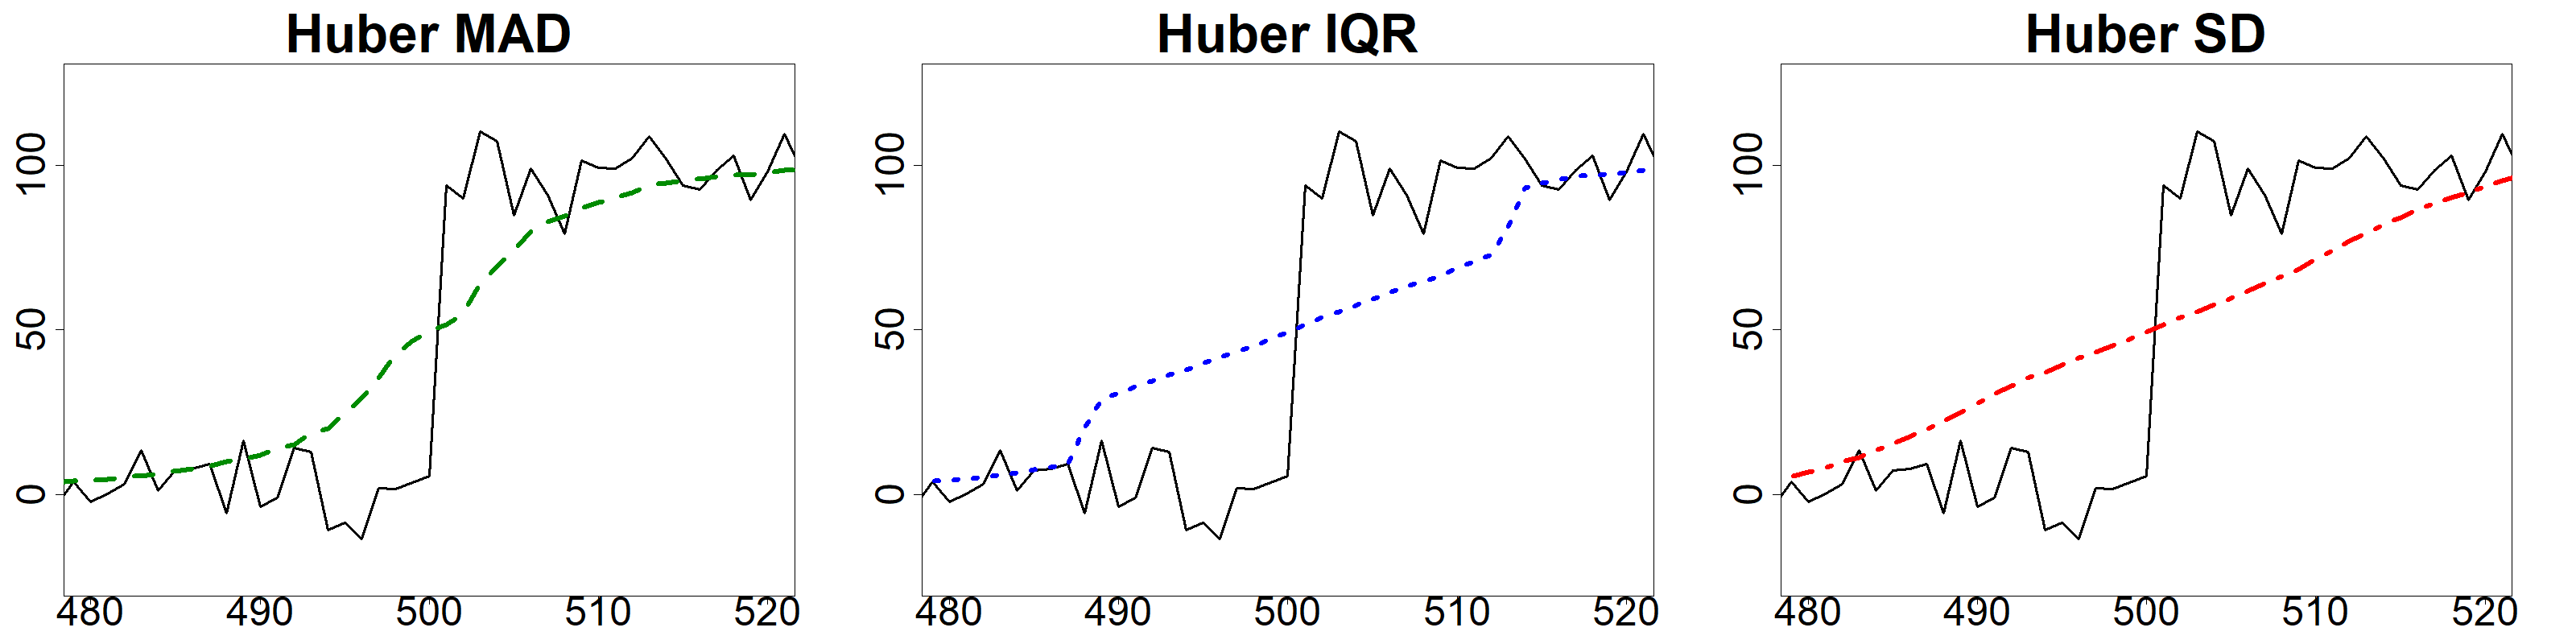
\includegraphics[width=\linewidth]{figures/3scale51.png}
        \caption{}
    \end{subfigure}
        
    \vspace{1em}
    
    \begin{subfigure}[b]{\linewidth}
        \centering
        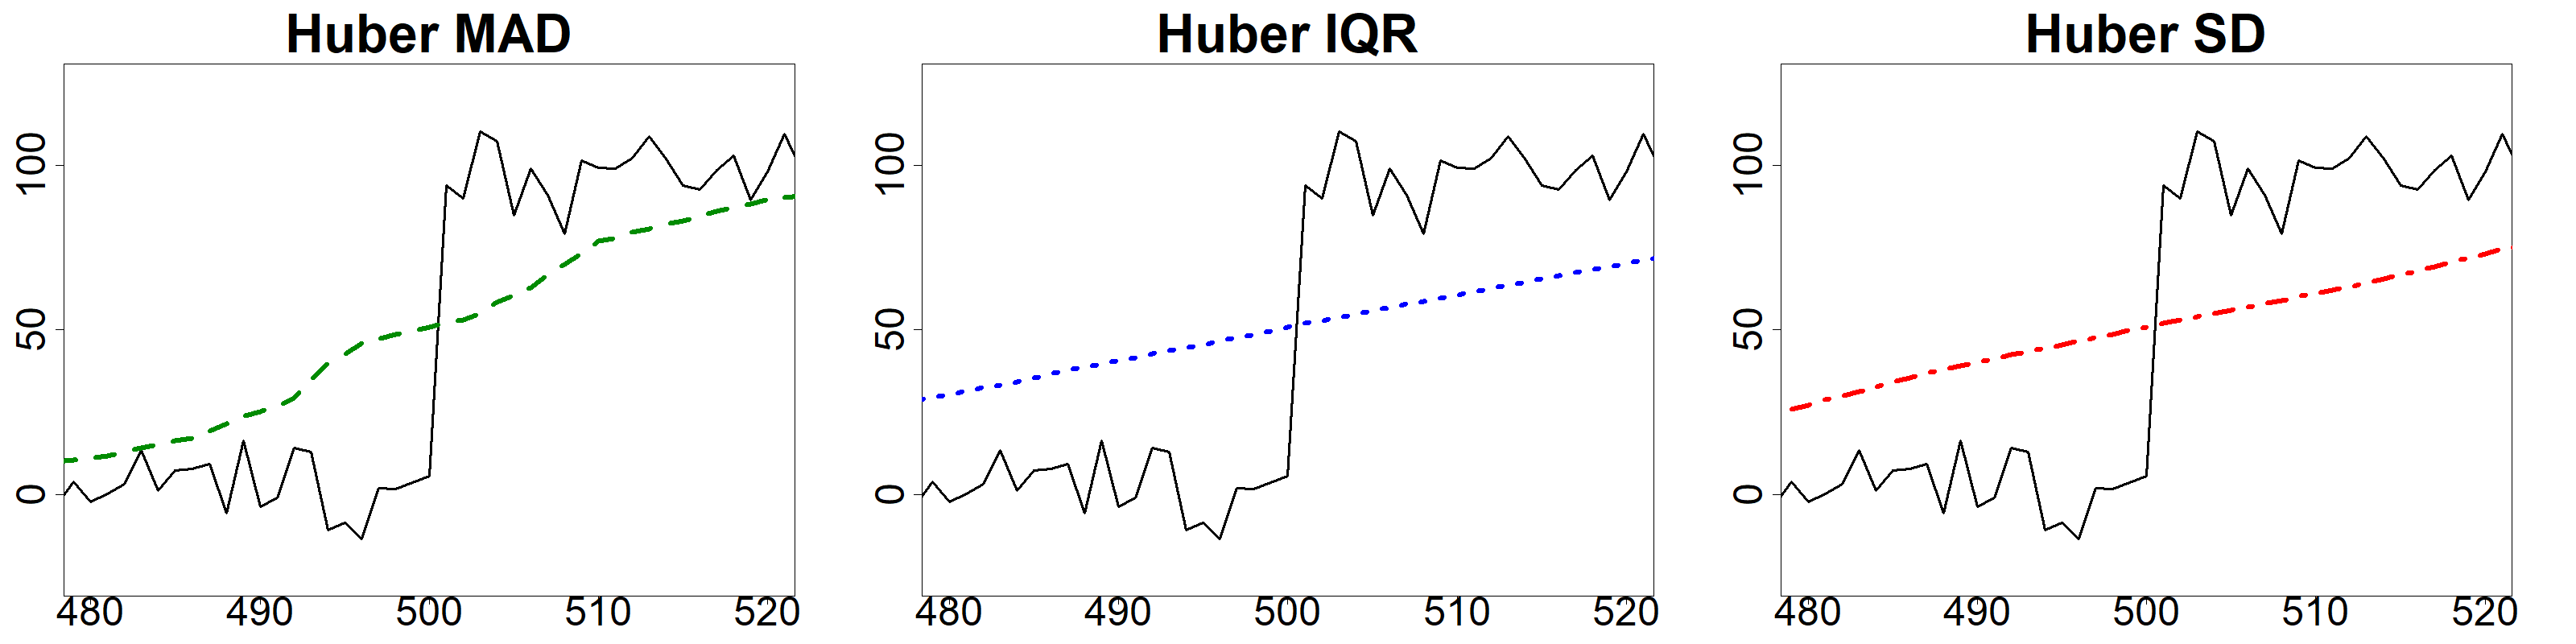
\includegraphics[width=\linewidth]{figures/3scale101.png}
        \caption{}
    \end{subfigure}
    
    \caption{점프 데이터에서의 세 가지 척도모수 추정 방법들의 비���}
    \label{fig:comparison}
\end{figure}
이 방법을 사용하게 되면, 창마다 중앙값을 한번만 계산하는 이동중앙값보다 정렬하는 계산비용이 훨씬 높아지게 된다. 따라서 MAD말고 IQR, SD, 또는 척도모수를 사용하지 않는 방법을 통해 이전 절과 동일한 데이터에 동일한 창으로 비교하였다.
Figure 3(a)에서 크게 차이는 안나지만, 자세히 보면 MAD, IQR, SD 방법 순으로 점프에 로버스트하여 점프가 있는 구간에서의 기울기가 미세한 차이를 보인다. Figure 3(b)그림에서는 IQR과 SD는 거의 동일하게 직선 형태를 띄며 이동평균과 유사한 반면, MAD는 부드러운 곡선 형태를 띈다. 창이 크기 때문에 3가지 방법 모두 점프라는 정보를 나타내진 못했지만, MAD가 점프에 더 로버스트한 것을 알 수 있다.

손실 함수는 이상점(outlier)에 의한 영향을 줄이고, 보다 로버스트한 추정을 가능하게 하는 중요한 도구이다. 전통적인 $L_2$ 손실 함수는 모든 잔차를 제곱함으로써 극단적인 이상점에 민감하게 반응하지만, Huber 손실 함수는 잔차가 작을 때는 제곱 손실을, 임계값을 초과하면 선형 손실을 적용하여 이상점의 영향을 완화한다. 이러한 특성 덕분에 Huber 손실 함수는 평가지표 측면에서 우수한 성능을 보이지만, 계산 비용이 증가하는 단점이 있다.

반면, Tukey와 Hampel 손실 함수는 redescending 특성을 활용하여 이상점의 영향력을 보다 적극적으로 차단하는 동시에, 척도 모수 추정을 통해 데이터의 분산 특성을 효과적으로 반영한다. 특히, 이들 함수는 MAD와 같은 로버스트한 척도 모수 추정 방식을 필수적으로 포함함으로써, IQR이나 SD 방식과 같이 평가지표와 실행시간 측면에서 각각 trade-off를 보이는 특성을 가지고 있다.

따라서, 본 연구에서는 Huber 손실 함수뿐만 아니라 Tukey 및 Hampel 손실 함수도 함께 비교하여, 응용 목적에 따라 어떤 방식이 보다 적절한지 평가하고자 하였다.

2.4절에서 사용했던 데이터를 100개의 시드로 $\sigma=1,10,20$ , $W=5,101$ 로 모의실험하여 실제 신호에 대한 $L_1$, $L_2$, $L_\infty$의 평균과 표준편차를 표1$\sim$6에 기입하였다.
기존 방법인 이동평균과 이동중앙값, 단순지수평활법, 손실함수(Huber, Tukey, Hampel)와 척도모수 추정 방법(MAD, IQR, SD)에 따른 여러가지 평가지표를 비교하였다. 
잔차를
\[
r_i = y_i - \hat y_i,\quad i = 1,2,\dots,n
\]
라 할 때, 평가지표 세 가지를

\[
\mathrm{L}_1
= \sum_{i=1}^n \bigl|r_i\bigr|,\;
\mathrm{L}_2 = \sqrt{\sum_{i=1}^n r_i^2},\;
\mathrm{L}_\infty = \max_{1 \le i \le n} \bigl|r_i\bigr|
\]

로 정의한다.
3개의 평가지표를 사용한 이유는 먼저 $L_1$은 절대 오차 합을 계산하므로 이상점이 일부 존재하더라도 비교적 안정적인 중앙값 형태의 오차를 보여주므로 전체적인 예측 정확도를 가늠할 수 있다. 반면 $L_2$는 제곱 오차에 대한 지표로, 이상점에 대해 가중치를 더 크게 부여하므로 모델이 극단적인 잔차까지 얼마나 잘 적합하는지를 평가하는데 효과적이다. 마지막으로 $L_\infty$는 모델이 기록한 최악 오차 하나만을 평가한다. 즉, 단일 극단 오차를 얼마나 억제하였는가를 측정하는 지표이다.

먼저 $\sigma=1$인 표 1,2에서, Hampel\_mad 방법이 모든 지표에서 가장 작은 값을 가진다. Tukey\_mad는 Hampel\_mad와 마찬가지로 이동중앙값보다 좋은 성능을 보여줬지만, Huber\_mad는 표1에서만 해당된다. 
Tukey\_mad와 Hampel\_mad는 redescending 특성으로 이상점의 영향을 잘 안받으면서 점프도 잘 보존한 것을 알 수 있다.
$L_\infty$ 값이 매우 작은 것을 보아, 점프를 잘 추정한 것을 알 수 있다. 그리고 척도 모수 방법들인 mad, iqr, sd를 비교했을땐 mad가 더 좋은 것을 알 수 있다.

$\sigma=10,20$이고 window=101일때, 이동중앙값이 모든 지표에서 압도적인 성능을 보여준다. 하지만 이동평균의 표준편차가 다른 방법들에 비해 유독 큰 것을 알 수 있다.
일반적으로 창의 크기가 작을 때, $\sigma$가 커질수록 지표들의 차이가 크지않고, SES의 $L_1$, $L_2$ 성능이 더 좋아진다. 하지만 $L_\infty$에선 SES가 가장 나쁘고 이동중앙값이 근소한 차이로 제일 좋다.

MAD가 IQR과 SD보다 모든상황에서 성능이 좋은것은 아니지만, 앞선 그래프와 성능지표를 살펴 봤을때 MAD 방법보단 부족하다고 판단하여 시뮬레이션 파트에서는 제거하였다.


%%%%%%%%%%%%%%%%%%%%%%%%%%%%%%%%%%%%%%%%%%%%%%%%%%%%%%%%%%%
% Table: Results for $\sigma=1$, window = 5
\begin{table}[H]
\small
\centering
\caption{$\sigma$ = 1, window = 5}
\vspace{-2mm}
\label{tab:s1w5}
\begin{tabular}{lccc}
\toprule
Method      & $L_1$             & $L_2$             & $L_\infty$       \\
\midrule
MA          & 476.8(17.98)      & 64.8(0.331)       & 40.34(0.277)     \\
MM          & 431(20.17)        & 17.14(0.741)      & 1.895(0.301)     \\
SES         & \textit{843.8(21.58)} & \textit{104.6(0.912)} & \textit{100(0.918)} \\
Huber\_mad  & 383.2(18.66)      & 15.51(0.779)      & 3.092(1.068)     \\
Huber\_iqr  & 452.8(17.93)      & 58.47(0.262)      & 40.34(0.277)     \\
Huber\_sd   & 468.9(17.85)      & 62.08(0.322)      & 40.34(0.277)     \\
Tukey\_mad  & 394.7(18.96)      & 15.78(0.72)       & 1.799(0.246)     \\
Tukey\_iqr  & 462.7(17.8)       & 57.38(0.27)       & 39.44(0.278)     \\
Tukey\_sd   & 465.4(17.92)      & 59.77(0.338)      & 38.56(0.281)     \\
Hampel\_mad & \textbf{376.1(18.67)} & \textbf{14.99(0.714)} & \textbf{1.707(0.266)} \\
Hampel\_iqr & 452(18.07)        & 58.47(0.259)      & 40.34(0.277)     \\
Hampel\_sd  & 476.8(17.98)      & 64.8(0.331)       & 40.34(0.277)     \\
\bottomrule
\end{tabular}
\end{table}
\vspace{-6mm}

%%%%%%%%%%%%%%%%%%%%%%%%%%%%%%%%%%%%%%%%%%%%%%%%%%%%%%%%%%%
% Table: Results for $\sigma=1$, window = 101
\begin{table}[H]
\small
\centering
\caption{$\sigma$ = 1, window = 101}
\vspace{-2mm}
\label{tab:s1w101}
\begin{tabular}{lccc}
\toprule
Method      & $L_1$             & $L_2$             & $L_\infty$       \\
\midrule
MA           & \textit{2607(17.18)}  & \textit{290.1(0.278)} & \textit{49.57(0.053)}   \\
MM           & 176.4(22.54)      & 10.08(1.204)      & 2.575(0.422)     \\
SES          & 843.8(21.58)      & 104.6(0.912)      & 100(0.918)       \\
Huber\_mad   & 253.4(23.96)      & 26.75(1.809)      & 10.36(1.094)     \\
Huber\_iqr   & 1985(17.38)       & 270.8(0.187)      & 49.57(0.053)     \\
Huber\_sd    & 2292(17.83)       & 273.2(0.251)      & 49.57(0.053)     \\
Tukey\_mad   & 103.6(19.56)      & 5.224(1.464)      & 1.064(0.589)     \\
Tukey\_iqr   & 1924(16.93)       & 264.6(0.186)      & 49.53(0.053)     \\
Tukey\_sd    & 2181(17.56)       & 262.5(0.258)      & 49.46(0.053)     \\
Hampel\_mad  & \textbf{98.38(18.79)}  & \textbf{4.815(1.327)}  & \textbf{1.063(0.59)}    \\
Hampel\_iqr  & 1970(16.74)       & 270.8(0.184)      & 49.57(0.053)     \\
Hampel\_sd   & 2515(17.14)       & 287.5(0.265)      & 49.57(0.053)     \\
\bottomrule
\end{tabular}
\end{table}

%%%%%%%%%%%%%%%%%%%%%%%%%%%%%%%%%%%%%%%%%%%%%%%%%%%%%%%%%%%
% Table: Results for $\sigma=10$, window = 5
\begin{table}[H]
\small
\centering
\caption{$\sigma$ = 10, window = 5}
\vspace{-2mm}
\label{tab:s10w5}
\begin{tabular}{lccc}
\toprule
Method      & $L_1$             & $L_2$             & $L_\infty$       \\
\midrule
MA           & 3688(179.8)       & 155.4(6.39)       & 43.38(2.77)      \\
MM           & \textit{4310(201.7)} & 171.4(7.41)       & \textbf{18.95(3.009)} \\
SES          & \textbf{3494(198.9)} & \textit{192.9(6.481)} & \textit{100.3(3.977)} \\
Huber\_mad   & 3831(186.7)       & 154.7(7.597)      & 29.7(8.321)      \\
Huber\_iqr   & 3808(179.4)       & 158.7(6.517)      & 43.34(2.74)      \\
Huber\_sd    & 3699(178.5)       & 155.1(6.451)      & 43.36(2.756)     \\
Tukey\_mad   & 3973(193.4)       & 160.8(7.909)      & 29.11(9.407)     \\
Tukey\_iqr   & 3923(178)         & 162.9(6.549)      & 42.34(2.778)     \\
Tukey\_sd    & 3697(179.2)       & \textbf{154.3(6.482)} & 41.66(2.816)     \\
Hampel\_mad  & 3809(190.7)       & 155.9(7.913)      & 36.53(7.768)     \\
Hampel\_iqr  & 3801(180.7)       & 158.6(6.519)      & 43.38(2.77)      \\
Hampel\_sd   & 3688(179.8)       & 155.4(6.39)       & 43.38(2.77)      \\
\bottomrule
\end{tabular}
\end{table}
\vspace{-6mm}

%%%%%%%%%%%%%%%%%%%%%%%%%%%%%%%%%%%%%%%%%%%%%%%%%%%%%%%%%%%
% Table: Results for $\sigma=10$, window = 101
\begin{table}[H]
\small
\centering
\caption{$\sigma$ = 10, window = 101}
\vspace{-2mm}
\label{tab:s10w101}
\begin{tabular}{lccc}
\toprule
Method      & $L_1$             & $L_2$             & $L_\infty$       \\
\midrule
MA           & \textit{3352(171.8)}  & \textit{292.7(3.1)} & 50.2(0.533)     \\
MM           & \textbf{1764(225.4)}  & \textbf{100.8(12.04)} & \textbf{25.75(4.218)} \\
SES          & 3494(198.9)       & 192.9(6.481)      & \textit{100.3(3.977)} \\
Huber\_mad   & 2323(217.1)       & 210.6(8.782)      & 50.19(0.535)     \\
Huber\_iqr   & 2921(173.7)       & 275.6(2.654)      & 50.2(0.533)      \\
Huber\_sd    & 3077(178.1)       & 275(3.04)         & 50.18(0.534)     \\
Tukey\_mad   & 1951(234)         & 199.3(10.13)      & 50.12(0.536)     \\
Tukey\_iqr   & 2757(169.4)       & 267.6(2.453)      & 50.15(0.534)     \\
Tukey\_sd    & 3001(176.2)       & 267.4(3.177)      & 50.08(0.538)     \\
Hampel\_mad  & 2426(219.6)       & 237.1(8.14)       & 50.2(0.533)      \\
Hampel\_iqr  & 2839(170.4)       & 275.2(2.564)      & 50.2(0.533)      \\
Hampel\_sd   & 3277(171.4)       & 290.2(2.984)      & 50.2(0.533)      \\
\bottomrule
\end{tabular}
\end{table}
\vspace{-6mm}

%%%%%%%%%%%%%%%%%%%%%%%%%%%%%%%%%%%%%%%%%%%%%%%%%%%%%%%%%%%
% Table: Results for $\sigma=20$, window = 5
\begin{table}[H]
\small
\centering
\caption{$\sigma$ = 20, window = 5}
\vspace{-2mm}
\label{tab:s20w5}
\begin{tabular}{lccc}
\toprule
Method      & $L_1$             & $L_2$             & $L_\infty$       \\
\midrule
MA          & 7255(359.5)       & \textit{290.9(13.4)} & 46.77(5.527)     \\
MM          & \textit{8619(403.4)} & 342.7(14.82) & \textbf{37.89(6.018)} \\
SES         & \textbf{5067(366.7)} & \textbf{262.9(12.14)} & \textit{100.3(5.435)} \\
Huber\_mad  & 7638(370.1)       & 305.4(14.16)      & 42.97(6.3)       \\
Huber\_iqr  & 7534(358.6)       & 301.8(13.56)      & 46.25(5.593)     \\
Huber\_sd   & 7288(356.9)       & 292(13.46)        & 46.52(5.5)       \\
Tukey\_mad  & 7944(382.9)       & 319.1(14.59)      & 43.15(6.097)     \\
Tukey\_iqr  & 7769(356.1)       & 311.5(13.57)      & 45.32(5.606)     \\
Tukey\_sd   & 7288(358.3)       & 291.7(13.48)      & 45.24(5.645)     \\
Hampel\_mad & 7583(375.6)       & 304.5(14.35)      & 45.17(6.318)     \\
Hampel\_iqr & 7524(361.9)       & 301.8(13.63)      & 46.55(5.413)     \\
Hampel\_sd  & 7255(359.5)       & 290.9(13.4)       & 46.77(5.527)     \\
\bottomrule
\end{tabular}
\end{table}
\vspace{-6mm}

%%%%%%%%%%%%%%%%%%%%%%%%%%%%%%%%%%%%%%%%%%%%%%%%%%%%%%%%%%%
% Table: Results for $\sigma=20$, window = 101
\begin{table}[H]
\small
\centering
\caption{$\sigma$ = 20, window = 101}
\vspace{-2mm}
\label{tab:s20w101}
\begin{tabular}{lccc}
\toprule
Method      & $L_1$             & $L_2$             & $L_\infty$       \\
\midrule
MA          & \textit{4181(343.5)} & \textit{300.9(7.791)} & 50.89(1.066)    \\
MM          & \textbf{3523(449.5)} & \textbf{200.4(23.55)} & \textbf{49.46(6.117)} \\
SES         & 5067(366.7)       & 262.9(12.14)      & \textit{100.3(5.435)} \\
Huber\_mad  & 3836(392)         & 275(12.69)        & 50.93(1.134)     \\
Huber\_iqr  & 3937(345.6)       & 287.6(7.803)      & 50.89(1.066)     \\
Huber\_sd   & 3971(356.5)       & 284.1(8.716)      & 50.89(1.068)     \\
Tukey\_mad  & 3739(407.1)       & 272.1(14.14)      & 50.87(1.142)     \\
Tukey\_iqr  & 3825(344.5)       & 281.4(8.04)       & 50.82(1.072)     \\
Tukey\_sd   & 3947(353.6)       & 281.4(8.901)      & 50.78(1.079)     \\
Hampel\_mad & 4011(377.7)       & 291(11.18)        & 50.93(1.131)     \\
Hampel\_iqr & 3994(340.7)       & 292.9(7.688)      & 50.89(1.066)     \\
Hampel\_sd  & 4129(343)         & 298.5(7.767)      & 50.89(1.068)     \\
\bottomrule
\end{tabular}
\end{table}
\vspace{-6mm}

%%%%%%%%%%%%%%%%%%%%%%%%%%%%%%%%%%%%%%%%%%%%%%%%%%%%
\clearpage

%% Chap 3
\section{모의실험}\label{sec:thms}
본 연구에서는 두 가지 경우에 대해 노이즈를 각각 다르게 입혀서 비교해보려고한다. 첫 번째 경우는  \cite{verbout1998parameter}의 실험 데이터 구성을 참고하였다. 경계가 다수 존재하게끔 3가지 함수들을 합쳐 Figure 4 왼쪽 그림에 나타냈다. 1/3은 굴곡이 제법 있는 사인함수, 1/3은 계단함수, 1/3은 절댓값 함수를 이용해 뾰족한 부분을 나타냈다. 두 번째 경우는 경계가 없는 간단한 선형 모델 $x^3$이다. Figure 4 오른쪽 그림이다.
\begin{figure}[H]
    \centering
    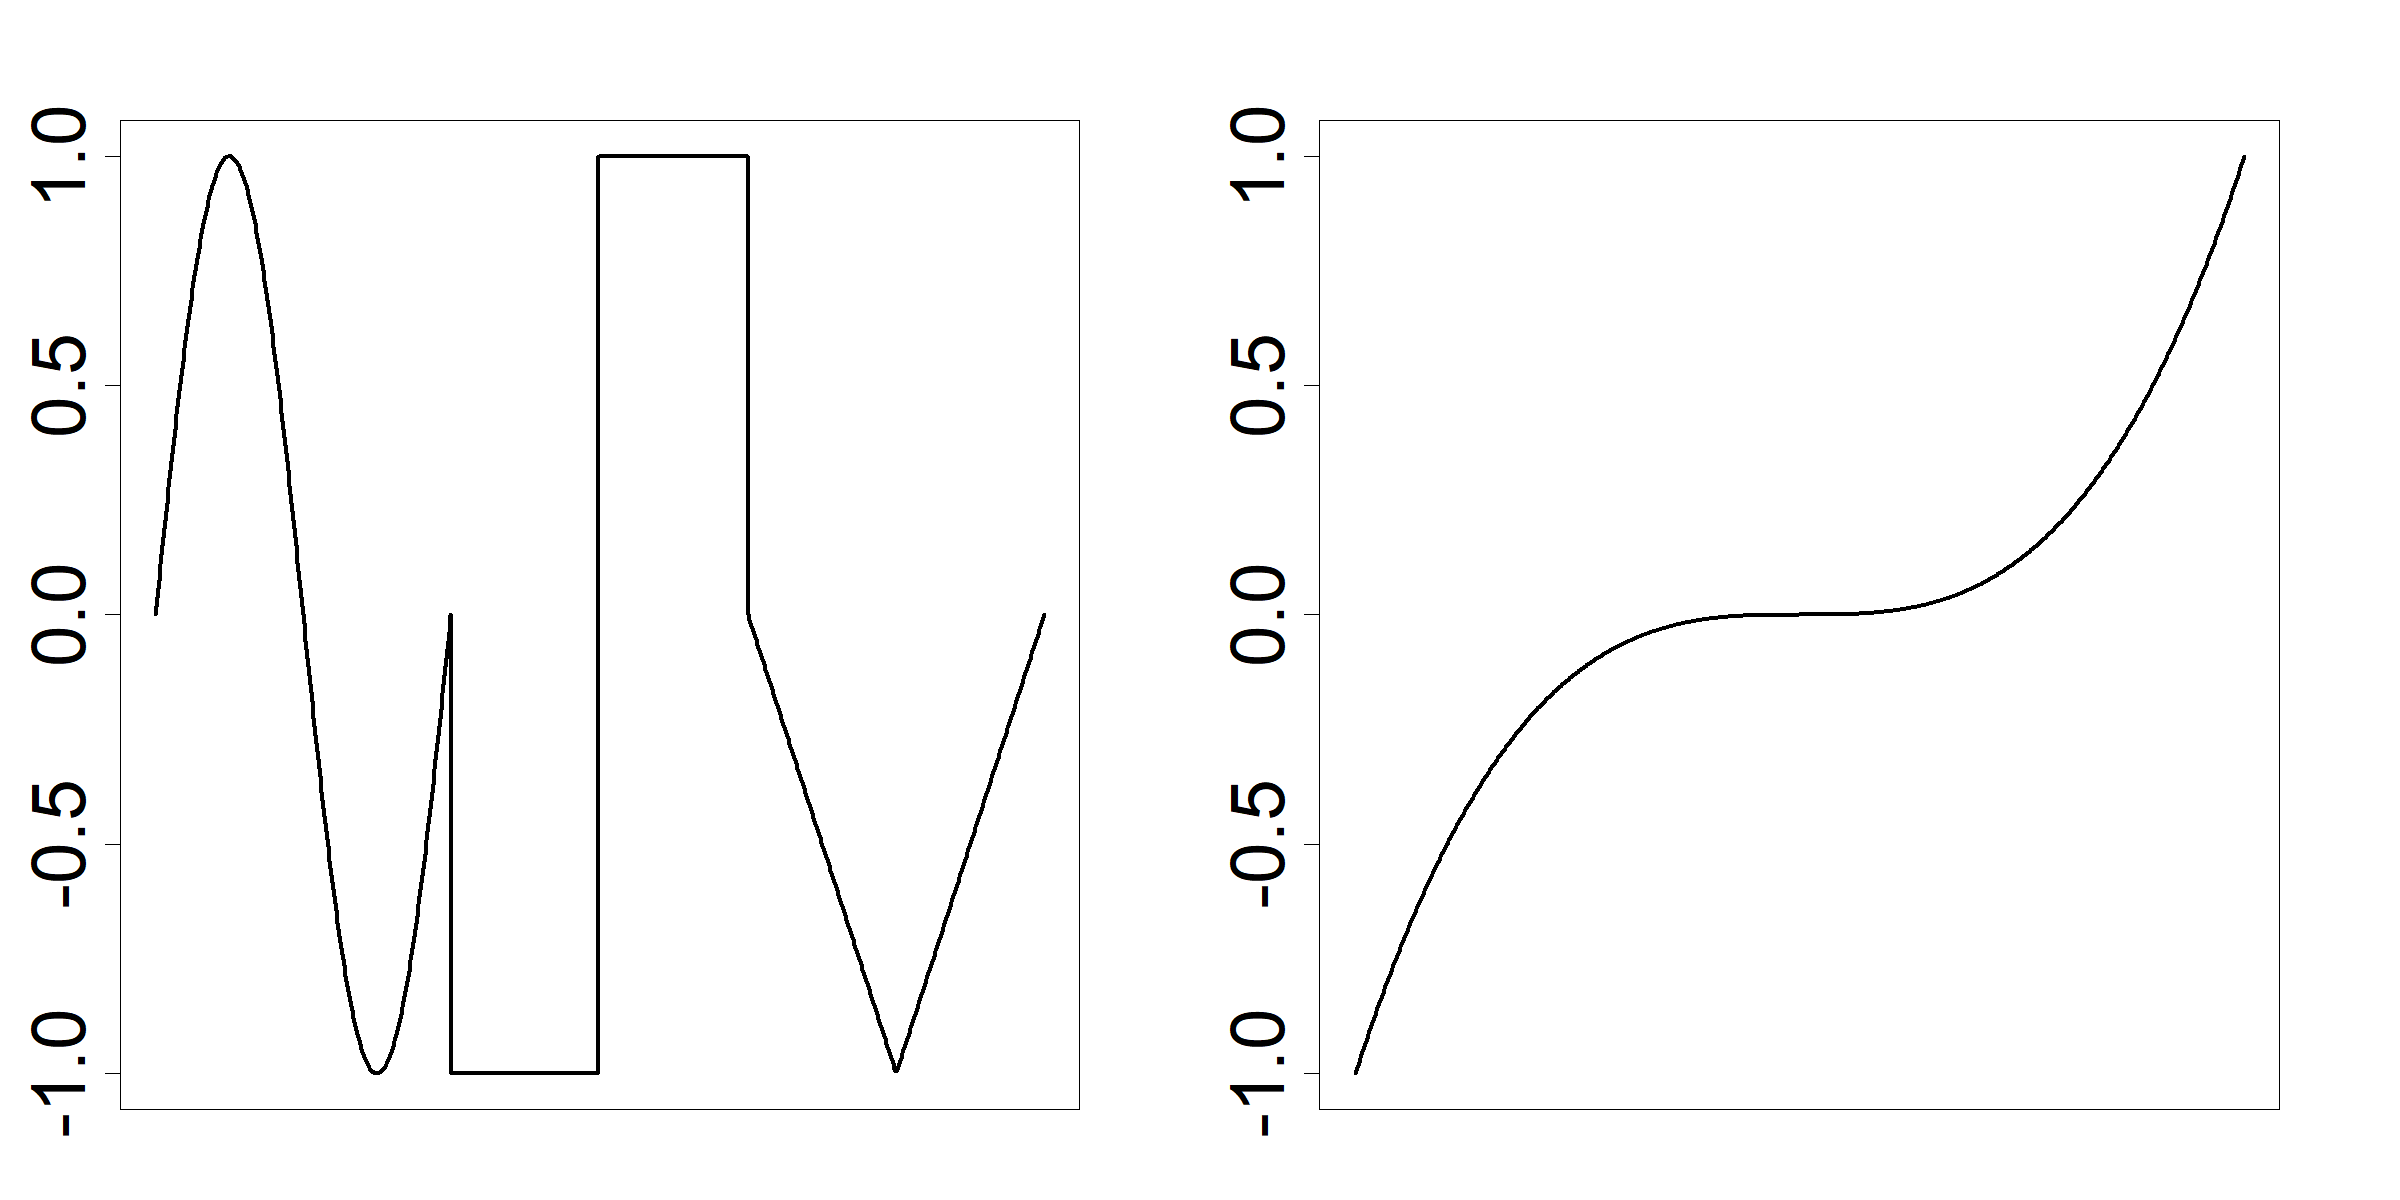
\includegraphics[width=0.8\linewidth]{figures/Truesignal.png}
    \caption{두 가지 형태의 신호. (왼쪽) 경계가 있는 신호, (오른쪽) 부드러운 신호}
\end{figure}
각각의 경우에 대해서 4가지 노이즈인 가우시안 노이즈, 라플라스 노이즈, 가우시안 혼합 노이즈, 코시 분포 노이즈를 사용했다.  \citet{verbout1998parameter} 에서는 가우시안 혼합 분포를 
\[
(\rho_1,\mu_1,\sigma_1)=(0.9,0.0,1.0) 
\]
\[
(\rho_2,\mu_2,\sigma_2)=(0.1,0.0,10.0)
\]

로 시그마와 10배의 시그마에 대해 0.9대 0.1 비율로 사용했다.
이것을 참고하여 가우시한 혼합 노이즈를 생성했다.
따라서 총 8개의 모델을 생성했다.
\[
f(t)=
\begin{cases}
\sin\!\Bigl(\dfrac{2\pi\,(t-1)}{332}\Bigr), & 1 \le t \le 333, \\[1mm]
-1, & 334 \le t \le 499, \\[1mm]
1, & 500 \le t \le 666, \\[1mm]
\Biggl|\,-1 + \dfrac{2(t-667)}{333}\Biggr| - 1, & 667 \le t \le 1000.
\end{cases}
\]
데이터의 함숫값의 범위는 $-1\le f(t) \le 1$이고 창 크기는 5로 고정했다. 대신 노이즈를 발생할때 사용하는 표준편차를 0.05,0.5,1,1.5 이 네가지로 분류했다. 100개의 시드값에 대해서 전부 계산한 후 각각의 노름에 대해 평균과 표준편차를 산출했다.

model1처럼 경계가 많은 데이터에 정규분포에 가까운 노이즈가 있을때, $M$-estimation 기반 추정량들이 좋은 성능을 보여주는데, 이동중앙값처럼 로버스트하면서도, 이동평균처럼 데이터의 분포를 잘 반영하기 때문이다.

model5,6,7 에서 모든 $\sigma$에 대해 SES가 모든 지표에서 가장 성능이 높게 나왔다. 신호가 부드럽게 변할 때는 SES가 신호의 전체적인 추세를 매우 잘 따라가기 때문에, 다른 방법들보다 정확하다.

코시 노이즈인  model8에서 모든 $\sigma$에 대해 $L_1,L_2$는 이동중앙값이, $L_\infty$에선 SES가 제일 좋은 성능을 보였다. 코시 노이즈는 극단적인 이상점이 있는 환경이므로 데이터의 순서를 이용해서 계산하는 이동중앙값이 강점을 보인다.


전체적으로, $\sigma$가 커져도 성능 순위는 크게 변하지 않는다. 또한 이동평균의 성능 지표값들이 다른 방법들에 비해 큰데, 이상점과 경계에 대한 제어가 잘 안되기 때문이다.


% --- sigma = 0.05, model = 1, window = 5 -------------------
\begin{table}[H]
\small
\centering
\caption{$\sigma$ = 0.05, model 1: 경계가 있는 신호에 가우시안 노이즈}
\label{tab:s5w5m1}
\begin{tabular}{lccc}
\toprule
Method         & $L_1$             & $L_2$             & $L_\infty$         \\
\midrule
MA             & 22.50(0.899)          & 1.706(0.018)          & 0.818(0.016)           \\
MM             & 21.88(0.995)          & 0.872(0.037)          & \textbf{0.102(0.016)}  \\
SES            & \textit{37.84(1.035)} & \textit{2.840(0.039)} & \textit{2.004(0.040)}  \\
Huber\_mad     & 19.64(0.949)          & 0.820(0.042)          & 0.197(0.047)           \\
Tukey\_mad     & 19.90(0.936)          & \textbf{0.801(0.037)} & 0.118(0.063)           \\
Hampel\_mad    & \textbf{19.20(0.960)} & 0.812(0.058)          & 0.247(0.101)           \\
\bottomrule
\end{tabular}
\end{table}

% --- sigma = 0.05, model = 5, window = 5 -------------------
\begin{table}[H]
\small
\centering
\caption{$\sigma$ = 0.05, model 5: 부드러운 신호에 가우시안 노이즈}
\label{tab:s5w5m5}
\begin{tabular}{lccc}
\toprule
Method         & $L_1$             & $L_2$             & $L_\infty$         \\
\midrule
MA             & 17.92(0.899)          & 0.710(0.034)          & 0.075(0.008)           \\
MM             & \textit{21.52(1.006)} & \textit{0.854(0.037)} & \textit{0.091(0.012)}  \\
SES            & \textbf{9.896(1.044)} & \textbf{0.391(0.040)} & \textbf{0.036(0.006)}  \\
Huber\_mad     & 18.96(0.926)          & 0.754(0.036)          & 0.084(0.013)           \\
Tukey\_mad     & 19.74(0.955)          & 0.789(0.037)          & 0.090(0.013)           \\
Hampel\_mad    & 18.80(0.947)          & 0.749(0.037)          & 0.085(0.014)           \\
\bottomrule
\end{tabular}
\end{table}

% --- sigma = 0.5, model = 8, window = 5 -------------------
\begin{table}[H]
\small
\centering
\caption{$\sigma$ = 0.5, model 8: 부드러운 신호에 코시 노이즈}
\label{tab:s50w5m8}
\begin{tabular}{lccc}
\toprule
Method         & $L_1$             & $L_2$             & $L_\infty$         \\
\midrule
MA             & \textit{3058(3233)}   & \textit{686.3(1387)}  & \textit{285.3(625.7)}  \\
MM             & \textbf{362.9(138.4)} & \textbf{31.59(131.9)} & 19.81(133.1)           \\
SES            & 1361(2294)            & 45.82(71.86)          & \textbf{2.365(2.326)}  \\
Huber\_mad     & 434.4(139.2)          & 35.59(131.5)          & 20.87(133.0)           \\
Tukey\_mad     & 395.0(137.3)          & 33.29(131.7)          & 20.20(133.0)           \\
Hampel\_mad    & 445.3(138.7)          & 36.37(131.4)          & 21.11(133.0)           \\
\bottomrule
\end{tabular}
\end{table}


% Chap 4
%%%%%%%%%%%%%%%%%%%%%%%%%%%%%%%%%%%%%%%%%%%%%%%%%%%%
\clearpage
\section{실제 데이터}\label{sec:examples}

\subsection{2021년도 게임스탑 고가 데이터}

본 절에서 고려한 데이터는 2021년도 게임스탑(GameStop)이라는 회사의 고가 주식 데이터로 야후파이낸스(Yahoo Finance)에서 데이터를 구하였다. 이 데이터의 시점은 2021년 1월 4일부터 2021년 12월 31일까지 하루 단위로 수집된 데이터이다. 1년 동안 대형 급등·급락 이벤트가 반복되어 경계가 뚜렷한 시계열이다. 

\begin{figure}[H]
    \centering
    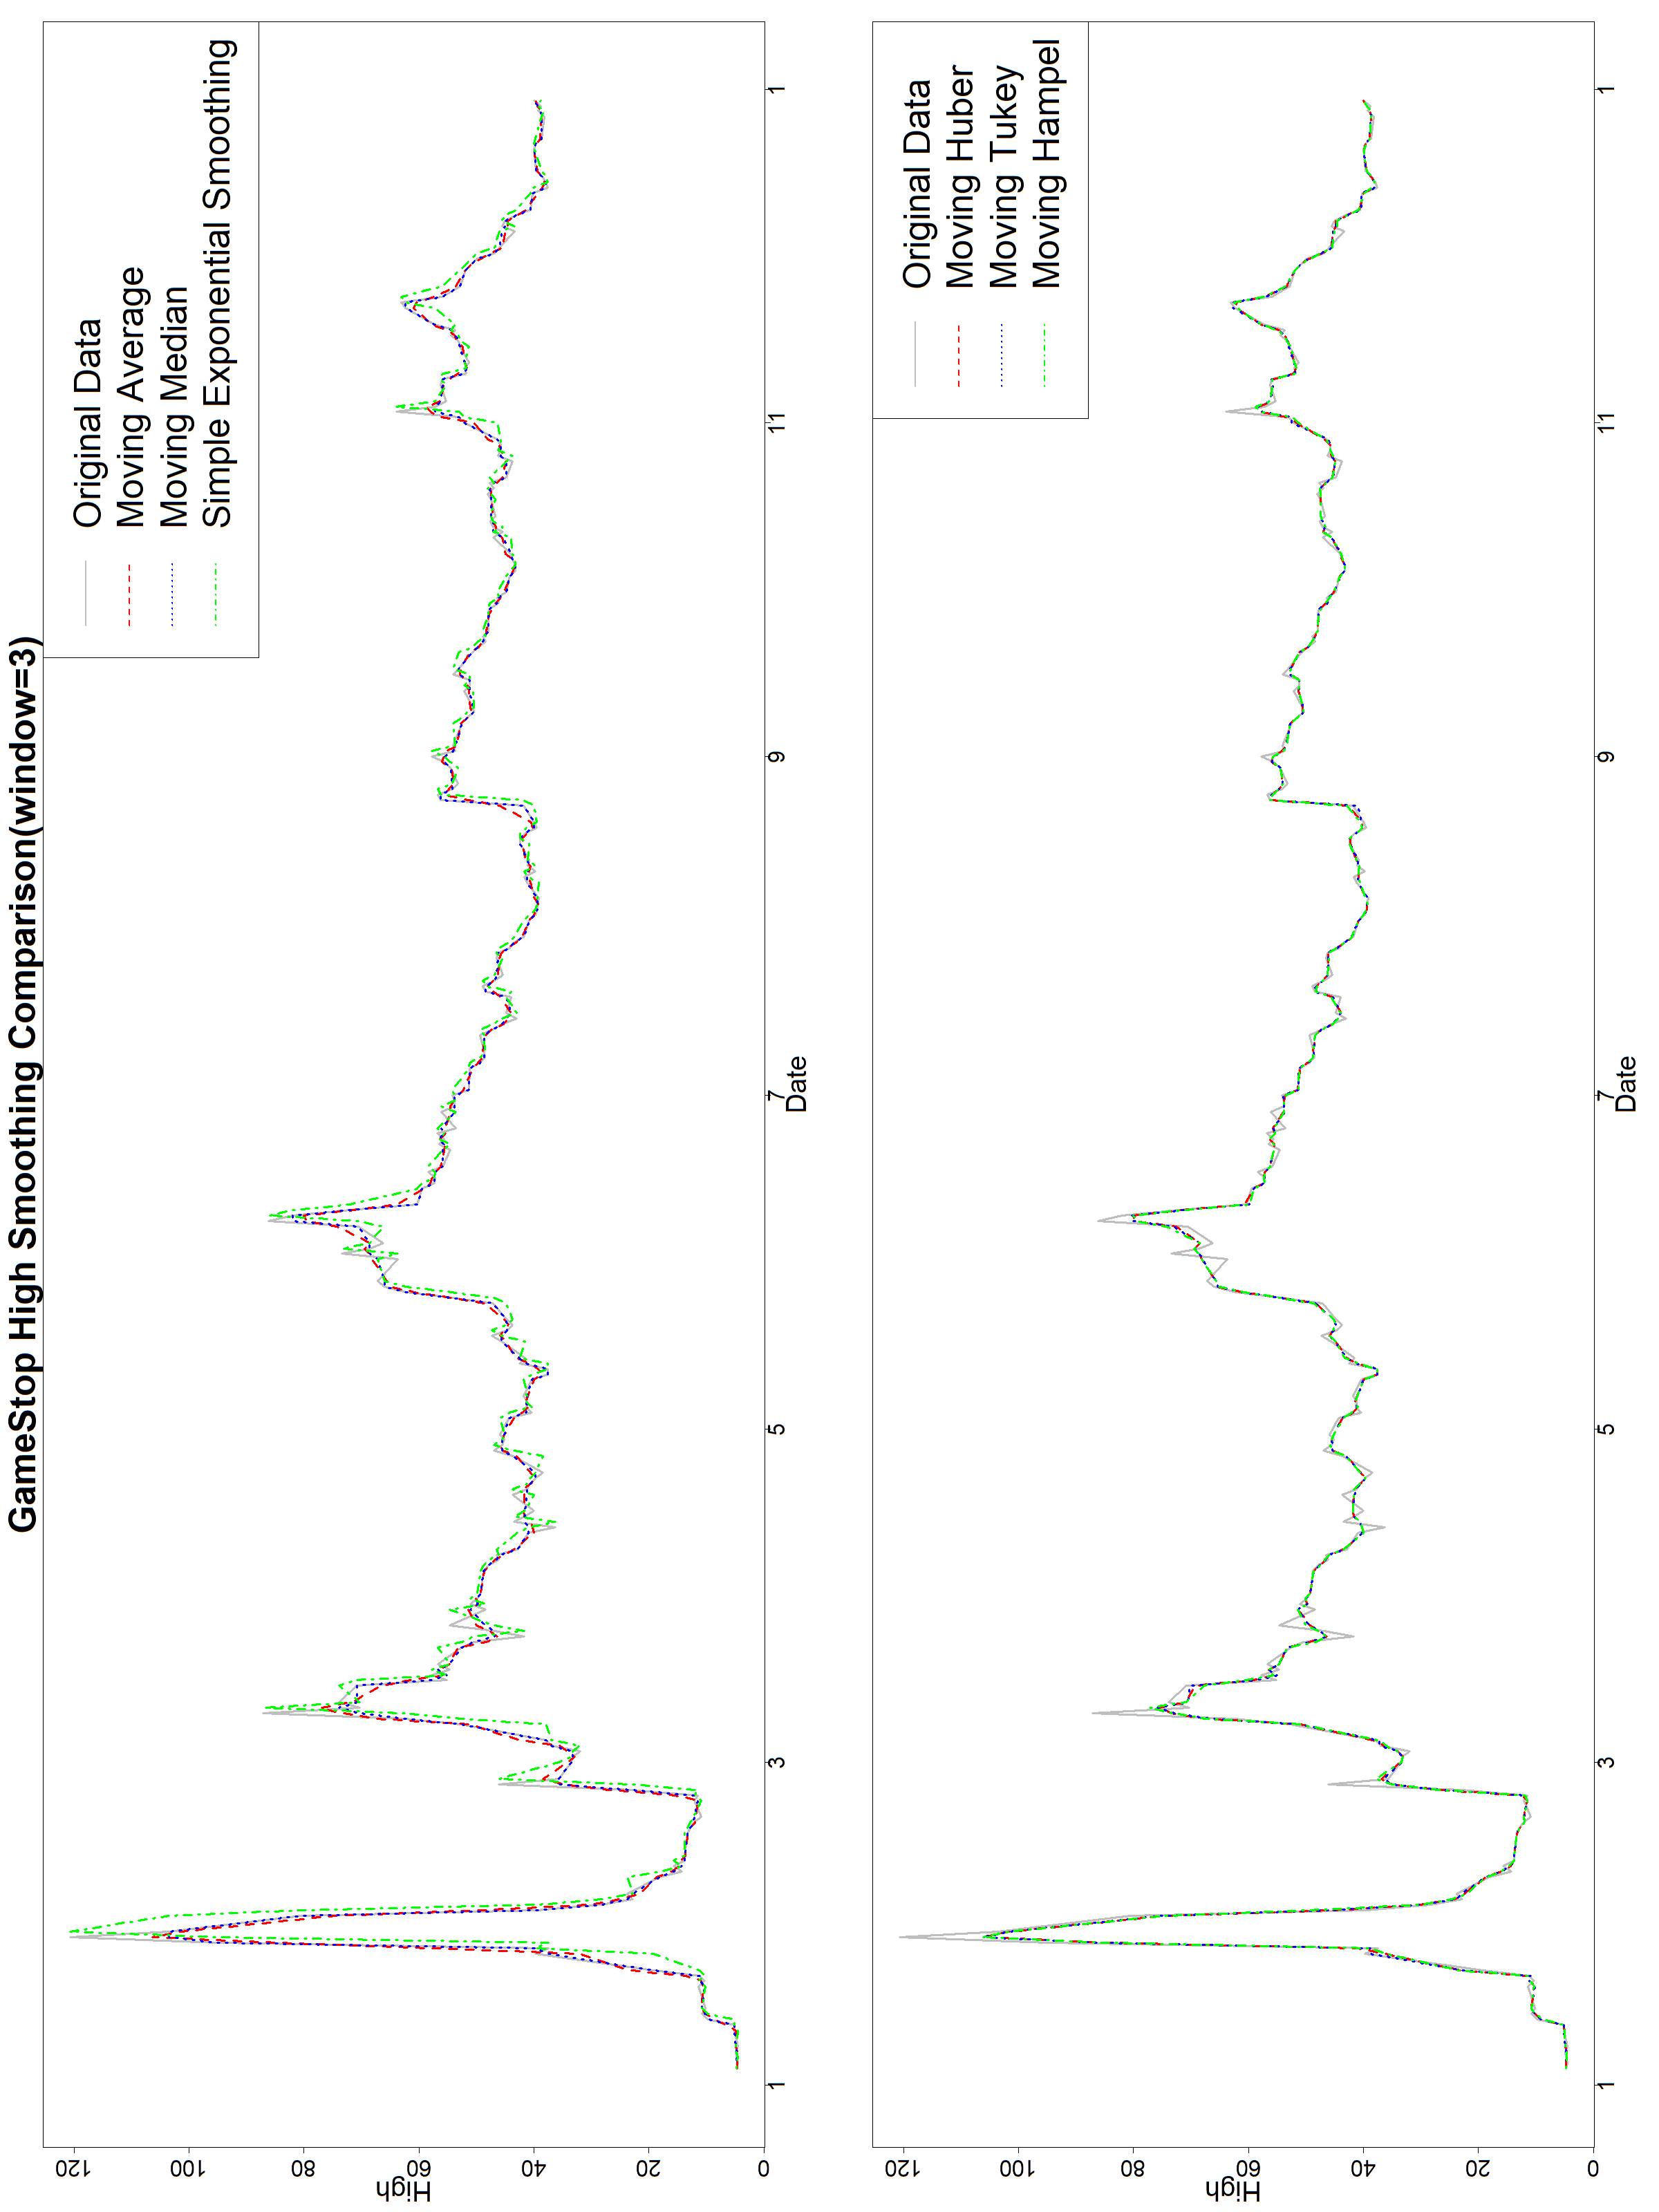
\includegraphics[width=1\linewidth]{figures/gamestop3_1.png}
    \caption{게임스탑 주식 그래프}
    \label{fig:enter-label}
\end{figure}

그림5의 상단 패널은 이동평균, 이동중앙값, SES 방법을 비교한다. 이동중앙값으로 디노이징한 값을 참값이라고 가정하자. SES는 급격한 경계에 민감해 일시적인 강인함이 관찰되나 그 차이는 크진 않다. 이동평균은 대부분의 경계에서 비교적 평활한 모습을 보였지만, $W$ 크기가 3이므로 그 정도가 크진 않다. 하단 패널의 Huber/Tukey/Hampel 도 중앙값에 가까운 동작을 하여 차이가 미세하다.

\subsection{도로 교통 센서 점유율}\label{subsec:TBM}
다음 데이터는 미국 미네소타 주 도심 고속도로의 차량 점유율 기록이다. 2015-09-01$\sim$2015-09-17 동안 약 30초 간격으로 수집된 약 2.4k 포인트 단일채널이다. 점유율은 해당 구간에 차량이 감지된 시간 비율로 정의된다.
\begin{figure}[H]
    \centering
    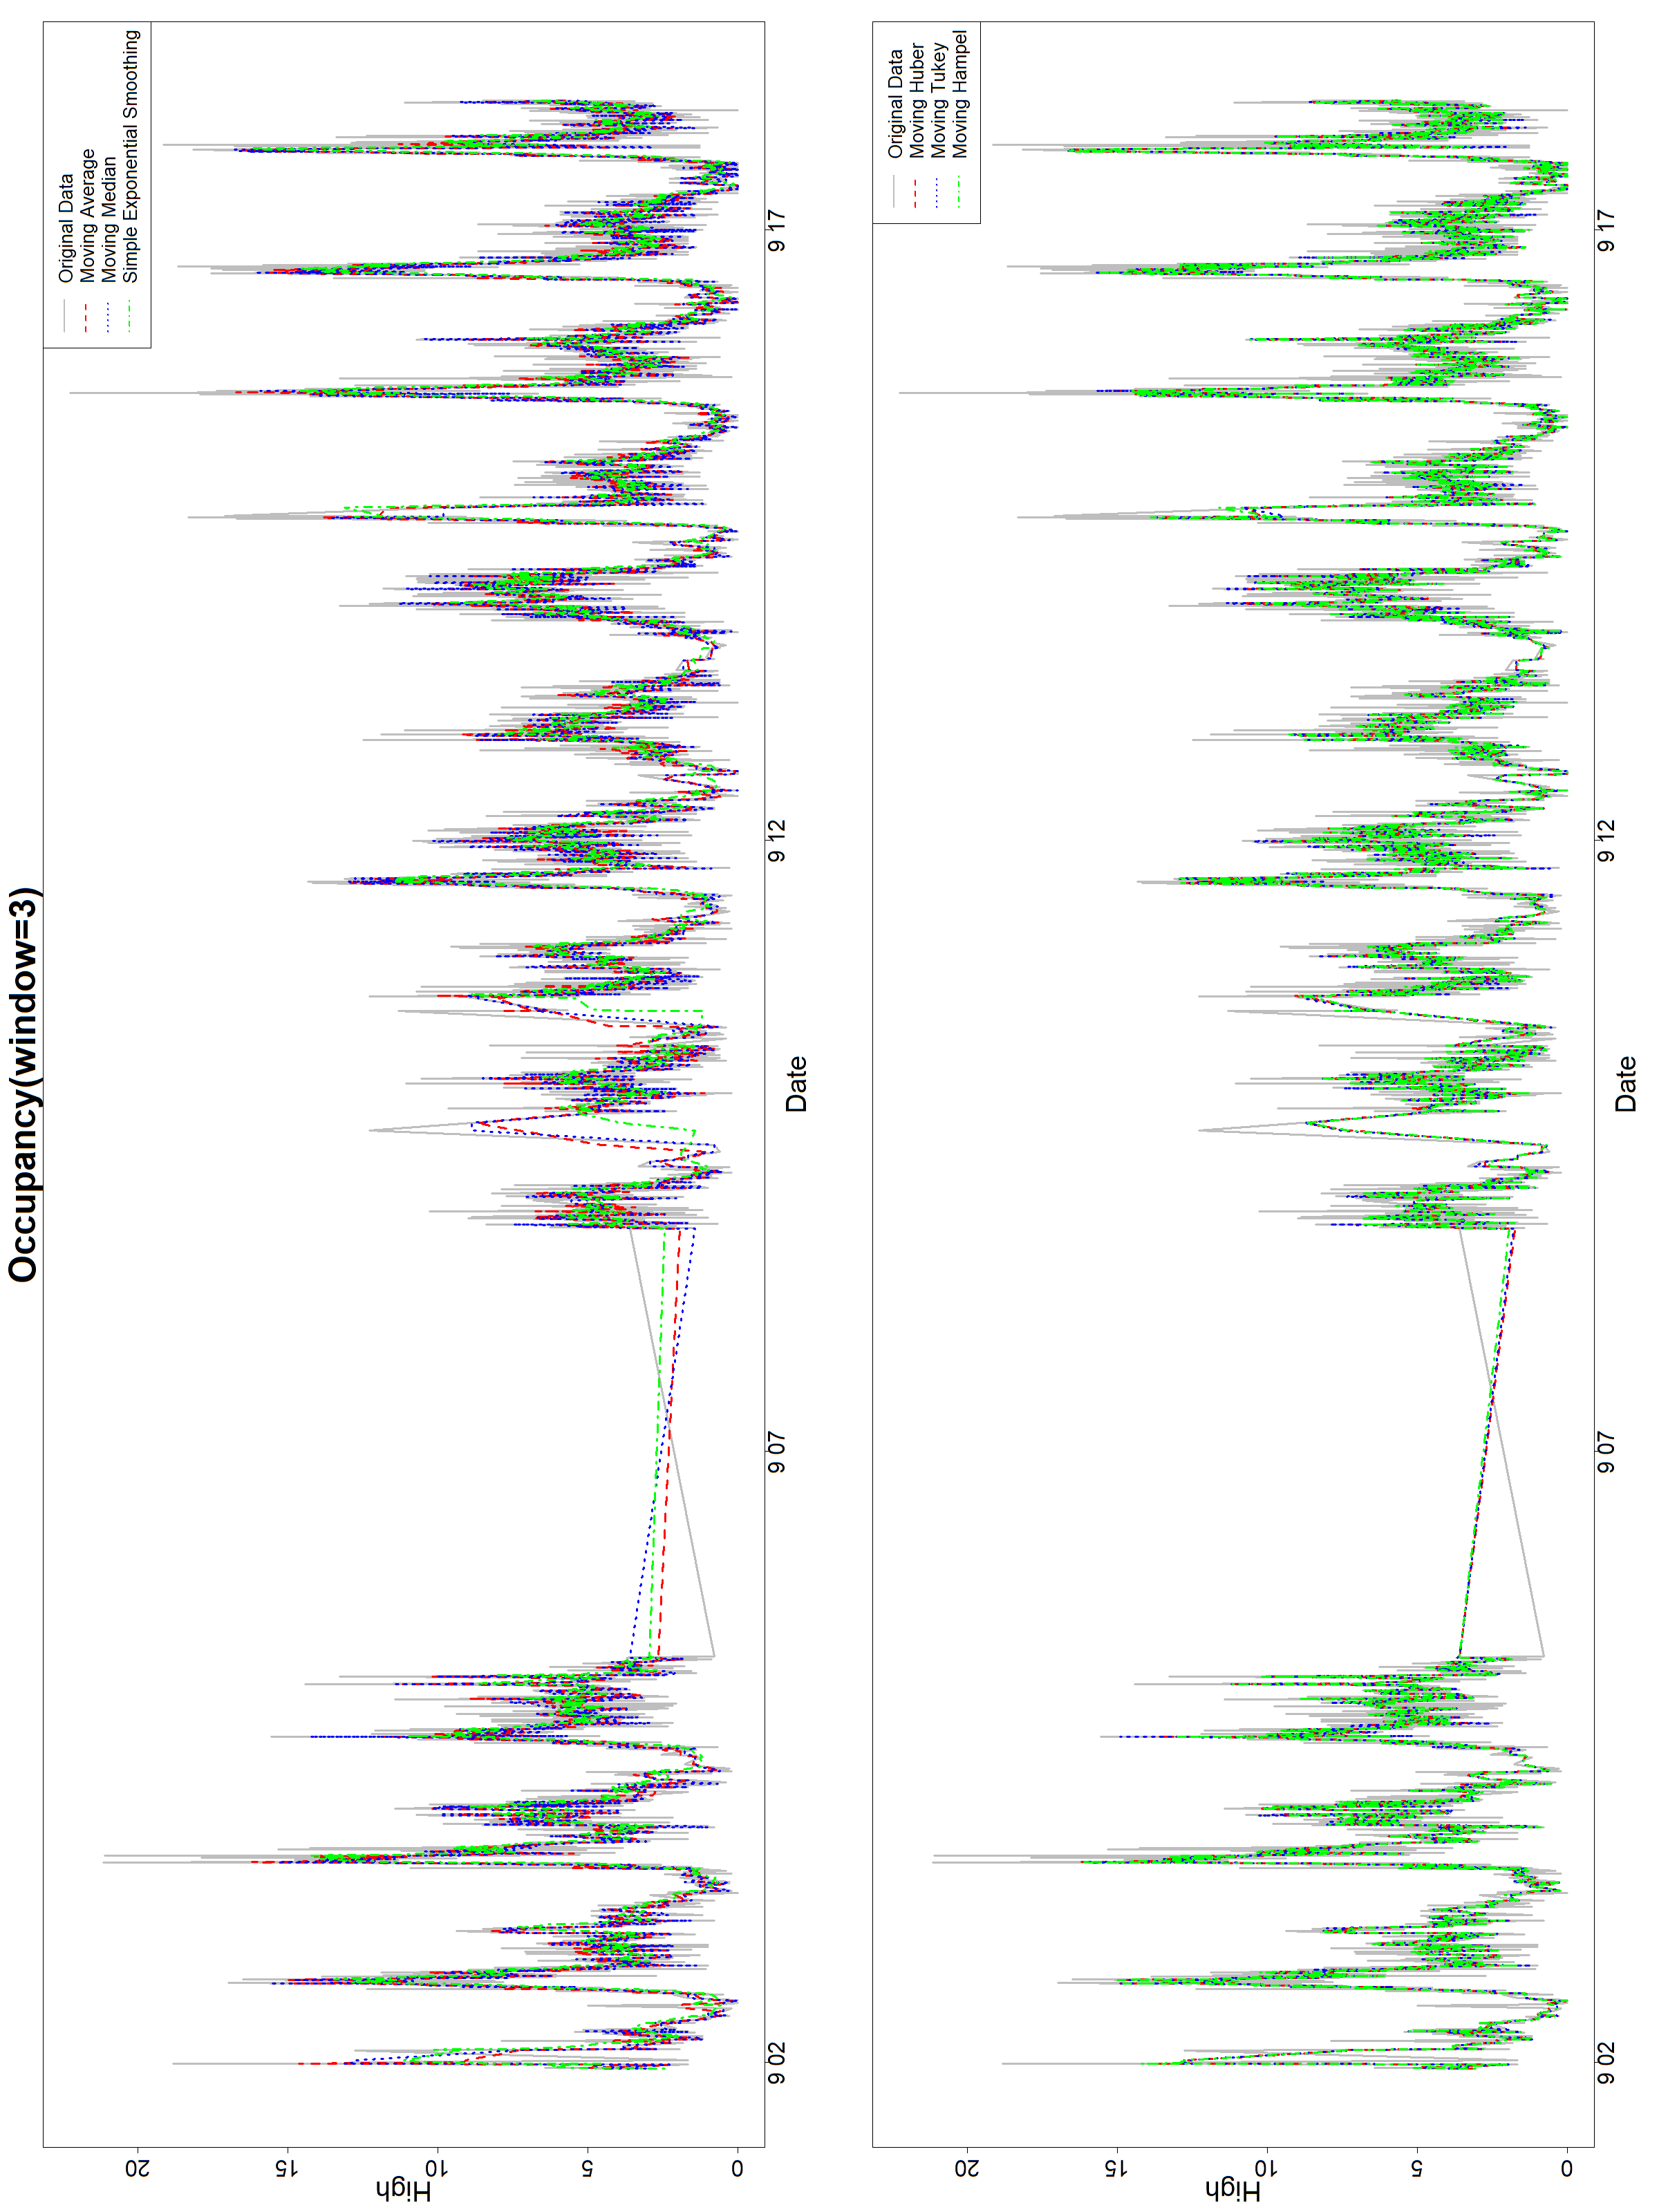
\includegraphics[width=1\linewidth]{figures/OCC_3_1.png}
    \caption{도로 교통 센서 점유율 그래프}
    \label{fig:enter-label}
\end{figure}
이 데이터는 주기성과 강한 변동을 확인할 수 있다. 이 데이터에서는 이동중앙값이 강인하게 디노이징했고, SES가 상대적으로 덜 강인하다. 밑 그림에선 Tukey 손실함수를 사용한 방법이 가장 강인하다.
\subsection{트위터 언급량}\label{subsec:TBM}
이 데이터는 트위터 상에서 특정 주제나 키워드 언급 횟수를 나타내는 시계열로, 대형 상장기업 Google에 대한 트윗 언급량이다. 5분마다 전 세계 트위터에서 'GOOG'라고 언급된 횟수를 집계한 것으로, 2015-02-26$\sim$2015-04-22 동안 총 15843개의 데이터 포인트가 있다.
\begin{figure}[H]
    \centering
    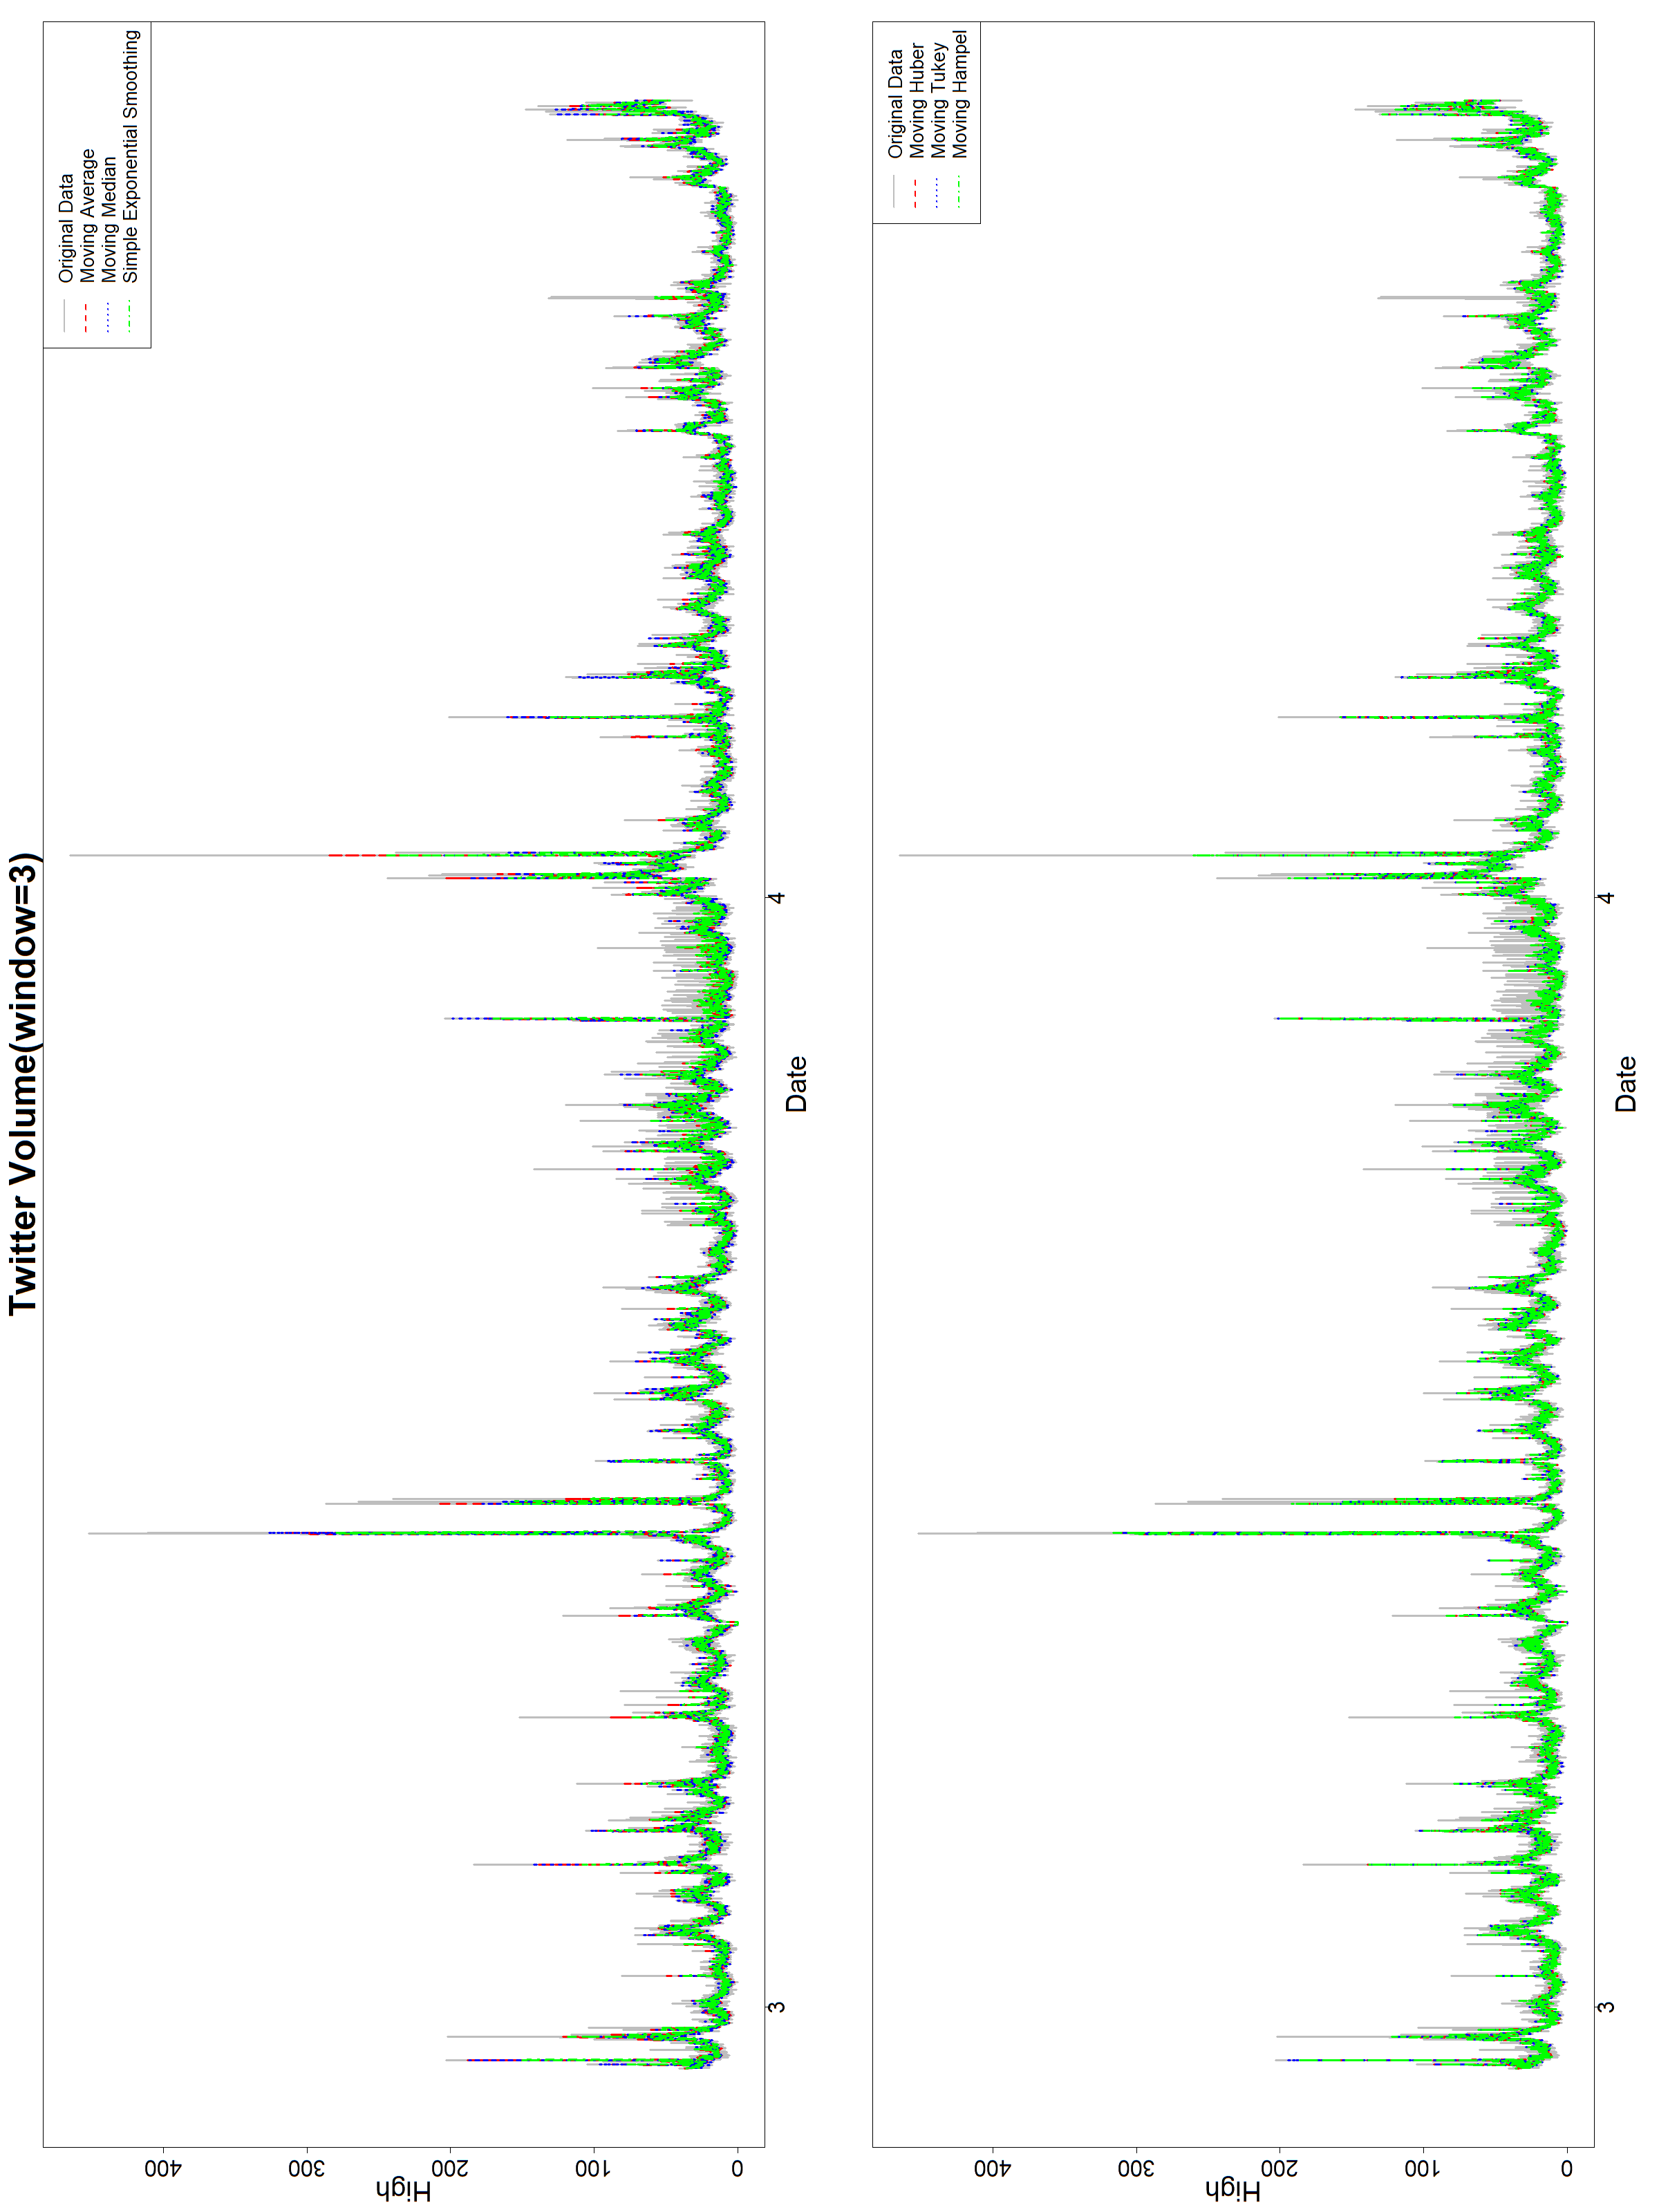
\includegraphics[width=1\linewidth]{figures/tw_3_1.png}
    \caption{트위터 언급량 그래프}
    \label{fig:enter-label}
\end{figure}
데이터 특징은 평범한 주기를 가지고있지만 매우 큰 슈팅이 나타난다는 것이다. 이동중앙값이 다른 이상점을 잘 찾는 것을 알 수 있다. 밑 그림에서의 3가지 방법들은 큰 차이 없이 비슷한 모습이다.


% Chap 5
%%%%%%%%%%%%%%%%%%%%%%%%%%%%%%%%%%%%%%%%%%%%%%%%%%%%
\clearpage
\section{결론}\label{sec:discuss}
본 연구는 시계열 데이터에 포함된 노이즈와 이상점을 효과적으로 제거하기 위한 디노이징 방법들을 비교 분석하였다. 특히 기존에 널리 사용되는 이동평균이 갖는 경계 정보 손실 문제와 이동중앙값이 갖는 계산 비용 문제를 보완할 대안으로, 이미지 처리 분야에서 제안된 $M$-smoother 방법을 시계열 데이터에 적용하고 그 성능을 종합적으로 비교 분석하였다.


%
모의실험을 통해 각 디노이징 방법의 성능을 다양한 실험 환경에서 확인한 결과, 데이터의 구조와 노이즈의 특성에 따라 최적의 방법이 달라짐을 확인할 수 있었다.
%

%
첫째, 신호에 경계가 존재하는 경우, 노이즈 수준이 낮을 때는 Tukey, Hampel 손실 함수를 사용한 $M$-estimation 기반 방법들이 이동평균보다 경계를 잘 보존하면서도 이동중앙값보다 부드러운 결과를 보여주며 가장 우수한 성능을 기록했다. 이는 $M$-estimation 방법이 이상점에 강건하면서도 데이터의 국소적인 분포를 반영하는 균형 잡힌 대안이 될 수 있음을 시사한다. 하지만 노이즈의 표준편차가 커지거나 창의 크기가 넓어질 경우, 이동중앙값의 강건성이 두드러져 경계 보존에 가장 효과적이었다. 둘째, 신호가 경계 없이 부드럽게 변하는 경우에는 단순지수평활법이 전반적인 추세를 가장 잘 포착하여 오차가 가장 작았다. 셋째, 코시 분포와 같이 극단적인 이상점을 포함하는 환경에서는 순서 통계량에 기반한 이동중앙값이 다른 방법들을 압도하는 성능을 보여주었다.
%

결론적으로, 단일 디노이징 방법이 모든 유형의 시계열 데이터에 최적인 것은 아니며, 분석하고자 하는 데이터의 특성을 먼저 파악하고 그에 맞는 방법론을 선택하는 것이 중요함을 확인했다. 본 연구에서 중점적으로 탐구한 $M$-estimation 기반의 방법들은 특히 신호의 경계를 보존하면서 노이즈를 제거해야 하는 상황에서 이동평균과 이동중앙값의 장점을 절충하는 효과적인 대안�� 될 수 있다는 가능성을 보여주었다.






\clearpage


\bibliographystyle{apalike}
\bibliography{Ref}

%\bibliographystyle{abbrv}  % 또는 abbrv, unsrt 등
%\bibliography{Ref}         % Ref.bib 파일 이름에 맞게


%%%%%%%%%%%%%%%%%%%%%%%%%%%%제목이랑 초록 (영문으로 작성)
\newpage
\thispagestyle{empty}
\begin{center}
\vspace{3.5cm}
\fontsize{14}{10} \selectfont{Comparative study on denoising methods for time series\\}
\vspace{1.5cm}
\fontsize{12}{10} \selectfont{Donghyeok Kim\\}
\vspace{1cm}
\fontsize{11}{10} \selectfont{Department of Statistics\\
The Graduate School\\
Pusan National University\\}
\vspace{1.5cm}
\fontsize{12}{10} \selectfont{Abstract\\}
\vspace{-\baselineskip}
\end{center}

\vspace{1cm}
This study investigates practical denoising alternatives for time series with abundant boundaries and outliers, addressing the over-smoothing of Moving Average (MA) and the computational/scalability limitations of Moving Median (MM). We define a windowed Moving Huber $M$-estimation (MH) by applying the image-processing idea of the $M$-smoother together with Huber $M$-estimation solved via Iteratively Reweighted Least Squares (IRLS). MH is compared against MA, MM, and Simple Exponential Smoothing (SES). In simulations, we consider (i) edge-rich signals and (ii) smooth linear signals, each contaminated by four noise types—Gaussian, Laplace, Gaussian mixture, and Cauchy—and evaluate performance with $L_1$, $L_2$, $L_\infty$ criteria. Extrapolation and practical relevance are further examined on real data: daily high prices of GameStop in 2021, freeway occupancy from a traffic sensor, and 5-minute counts of “GOOG” mentions on Twitter. Results show no universally superior method: MH excels when boundaries are present and noise is modest; SES yields the best accuracy for smoothly varying signals; and MM is particularly effective under heavy-tailed contamination resembling Cauchy noise. These findings support method selection based on signal/noise regimes and suggest windowed MH as a viable alternative that complements the strengths and weaknesses of MA and MM.



\newpage
\thispagestyle{empty}
\begin{center}
\fontsize{0.1}{1} \selectfont{ㅁ}
\end{center}






\end{document}


\end{document}